%!TEX TS-program = xelatex
%!TEX encoding = UTF-8 Unicode
\documentclass[16pt,a4paper]{article}
\usepackage{fontspec,xltxtra,xunicode}
\usepackage[top=1.5in,bottom=1in,left=1.5in,right=1.5in]{geometry}
\usepackage{polyglossia}
\newfontfamily\thaifont{TH Sarabun New}
\setmainfont{TH Sarabun New}
\setdefaultlanguage{thai}
\XeTeXlinebreaklocale 'th'
\usepackage{scrextend}
\changefontsizes[20pt]{16pt}
\XeTeXlinebreakskip = 0pt plus 1pt
\defaultfontfeatures{Scale=1.23}
\renewcommand{\baselinestretch}{1.2}

\newcommand{\ThesisProposalTH}{โครงร่างวิทยานิพนธ์}
\newcommand{\ThesisProposalEN}{Thesis Proposal}
\newcommand{\ThesisTopic}{หัวข้อวิทยานิพนธ์}

% - - - - - - - - - - - - - - - - - - - -
% Control words
% - - - - - - - - - - - - - - - - - - - -
\newcommand{\scg}{กราฟการเรียกเชิงสถิต}
\newcommand{\scgEN}{Static call graph}

\newcommand{\cfg}{กราฟการไหลของการควบคุม}
\newcommand{\cfgen}{Control flow graph}

\newcommand{\DDPath}{DD-Path}
\newcommand{\DDPathEN}{Decision-to-decision Path}

\newcommand{\FeasiblePath}{เส้นทางที่เป็นไปได้}
\newcommand{\FeasiblePathEN}{Feasible path}

\newcommand{\InfeasiblePath}{เส้นทางที่เป็นไปไม่ได้}
\newcommand{\InfeasiblePathEN}{Infeasible path}

\newcommand{\FeasibleAndInfeasiblePath}{เส้นทางที่เป็นไปได้และไม่ได้}
\newcommand{\FeasibleAndInfeasiblePathEN}{Feasib/Users/sitdh/Desktop/vector-Overwatch-Ana-wallpaper.jpg Infeasible path}

\newcommand{\sourcecode}{รหัสต้นฉบับ}

\newcommand{\TestDataGeneration}{การสร้างข้อมูลทดสอบ}
\newcommand{\TestDataGenerationEN}{Test data generation}

\newcommand{\RegressionTesting}{การทดสอบเชิงทดถอย}
\newcommand{\RegressionTestingEN}{Regression testing}

\newcommand{\Repository}{คลังข้อมูล}
\newcommand{\RepositoryEN}{Repository}

\newcommand{\softwareComponent}{ส่วนประกอบซอฟต์แวร์}
\newcommand{\softwareComponentEN}{Software component}

\newcommand{\IntegrationTesting}{การทดสอบผสาน}
\newcommand{\IntegrationTestingEN}{Integration testing}

\newcommand{\class}{คลาส}
\newcommand{\classEN}{Class}

\newcommand{\method}{\mbox{เมท็อด}}
\newcommand{\methodEN}{Method}

\newcommand{\attribute}{แอททริบิวต์}
\newcommand{\attributeEN}{Attribute}

\newcommand{\MethodSignature}{ลายเซ็นของเมธอด}
\newcommand{\MethodSignatureEN}{Method signature}

\newcommand{\DirectedMultiGraph}{กราฟหลายทางมีทิศทาง}
\newcommand{\DirectedMultiGraphEN}{Directed multigraph}

\newcommand{\DirectedGraph}{กราฟมีทิศทาง}
\newcommand{\DirectedGraphEN}{Directed graph}

\newcommand{\ProgramGraph}{กราฟโปรแกรม}
\newcommand{\ProgramGraphEN}{Program graph}

\newcommand{\BasisPath}{เส้นทางมูลฐาน}
\newcommand{\BasisPathEN}{ฺBasis paths}

\newcommand{\Node}{โหนด}
\newcommand{\NodeEN}{Node}

\newcommand{\Edge}{เส้นเชื่อม}
\newcommand{\EdgeEN}{Edge}

\newcommand{\PredicateNode}{{\Node}เงื่อนไขการดำเนินงาน}
\newcommand{\PredicateNodeEN}{Predicate node}

\newcommand{\TestPath}{เส้นทางทดสอบ}
\newcommand{\TestPathEN}{Test path}

\newcommand{\sourcenode}{โหนดต้นทาง}
\newcommand{\sourcenodeEN}{Source node}

\newcommand{\sinknode}{โหนดปลายทาง}
\newcommand{\sinknodeEN}{Sink node}

\newcommand{\Cyclomatic}{ความซับซ้อนไซโคลเมทิก}
\newcommand{\CyclomaticEN}{Cyclomatic Complexity}

\newcommand{\inputVector}{เวกเตอร์นำเข้า}
\newcommand{\inputVectorEN}{Input vector}

\newcommand{\CUT}{{\class}ภายใต้การทดสอบ}
\newcommand{\CUTEN}{Class under test}

\newcommand{\SUT}{ซอฟต์แวร์ภายใต้การทดสอบ}
\newcommand{\SUTEN}{Software under test}

\newcommand{\Path}{ทางเดิน}
\newcommand{\PathEN}{Path}

\newcommand{\DynamicInformation}{ข้อมูลเชิงพลวัต}
\newcommand{\DynamicInformationEN}{Dynamic information}

\newcommand{\StaticInformation}{ข้อมูลเชิงสถิต}
\newcommand{\StaticInformationEN}{Static information}

\newcommand{\testSuite}{ชุดทดสอบ}
\newcommand{\testSuiteEN}{Test suite}

\newcommand{\testCase}{กรณีทดสอบ}
\newcommand{\testCaseEN}{Test case}

\newcommand{\Package}{โปรแกรมสำเร็จ} % http://www.rirs3.royin.go.th
\newcommand{\PackageEN}{Package}

\newcommand{\expectedOutput}{ผลลัพธ์ที่คาดหวัง}
\newcommand{\expectedOutputEN}{Expected output}

\newcommand{\csp}{ปัญหาการหาค่าเหมาะที่สุดเชิงการจัด} % https://www.cp.eng.chula.ac.th/~somchai/CD/2110427/2546/demo/HW2-TSP/saTSP.htm
\newcommand{\cspEN}{Constraint satisfaction problem}

\newcommand{\Algorithm}{ขั้นตอนวิธี}
\newcommand{\AlgorithmEN}{Algorithm}

\newcommand{\software}{ซอฟต์แวร์}
\newcommand{\softwareEN}{Software}

\newcommand{\tester}{นักทดสอบซอฟต์แวร์}
\newcommand{\testerEN}{Software tester}

\newcommand{\constantExtracting}{การรวบรวมค่าคงที่}
\newcommand{\constantExtractingEN}{Constant extracting}

\newcommand{\graphCreation}{การสร้างกราฟ}
\newcommand{\graphCreationEN}{Graph creation}

\newcommand{\sourcecodeInstrumention}{แทรกคำสั่งในรหัสต้นฉบับ}
\newcommand{\sourcecodeInstrumentionEN}{Source code instrumentation}

\newcommand{\testcaseGeneration}{การสร้างกรณีทดสอบ}
\newcommand{\testcaseGenerationEN}{Test case generation}

\newcommand{\testpathSelection}{การเลือกทางเดินทดสอบ}
\newcommand{\testpathSelectionEN}{Test path selection}

\newcommand{\randomTestData}{สุ่มข้อมูลนำเข้า}
\newcommand{\randomTestDataEN}{Random test data}

\newcommand{\testData}{ข้อมูลทดสอบ}
\newcommand{\testDataEN}{Test data}

\newcommand{\testCaseGeneration}{การสร้างกรณีทดสอบ}
\newcommand{\testCaseGenerationEN}{Test case generation}

\newcommand{\expectedOutputAdjustment}{การปรับค่าคาดหวัง}
\newcommand{\expectedOutputAdjustmentEN}{Expected output adjustment}

\newcommand{\executeSoftwareTesting}{ดำเนินการทดสอบซอฟต์แวร์}
\newcommand{\executeSoftwareTestingEN}{Software testing execute}

\newcommand{\testResultCompare}{เปรียบเทียบผลลัพธ์การดำเนินงาน}
\newcommand{\testResultCompareEN}{Compare test excution result}

\newcommand{\pathConditions}{เงื่อนไขของเส้นทาง}
\newcommand{\enum}{อีนัม}

\usepackage{indentfirst}
\usepackage{graphicx}
\graphicspath{ {figures/} }
\usepackage{titlesec}
\usepackage{pdflscape}

\titleformat{\section}{\bfseries}{\thesection}{1em}{}

\setlength\parindent{0.5in}
\setlength\parskip{.5em}
\titlespacing\section{0pt}{12pt plus 4pt minus 2pt}{0pt plus 2pt minus 2pt}
\titlespacing\subsection{0pt}{12pt plus 4pt minus 2pt}{0pt plus 2pt minus 2pt}
\titlespacing\subsubsection{0pt}{12pt plus 4pt minus 2pt}{0pt plus 2pt minus 2pt}

\newcommand{\makethesiscover}{ %

    \thispagestyle{empty}
    \begin{center}
        \bf
        {\large {\ThesisProposalTH} \\ ({\ThesisProposalEN})}
    \end{center}

    \noindent
    \begin{table}[ht!]
        \centering
        \label{tab:metadata}
        \begin{tabular*}{\linewidth}{ll@{\extracolsep{\fill}}}
            {\bf ชื่อเรื่อง (ภาษาไทย)}      & \ifdefined\ThesisThaiName \ThesisThaiName\fi          \\
            {\bf ชื่อเรื่อง (ภาษาอังกฤษ)}    & \ifdefined\ThesisEnglishName \ThesisEnglishName\fi    \\ \\
            {\bf เสนอโดย}               & \ifdefined\studentname \studentname\fi                \\
            {\bf รหัสนิสิต}                & \ifdefined\studentid \studentid\fi                    \\
            {\bf หลักสูตร}                & \ifdefined\curriculumn \curriculumn\fi                \\
            {\bf สาขา}                  & \ifdefined\major \major\fi                            \\
            {\bf ภาควิชา}                & \ifdefined\department \department\fi                  \\
            {\bf คณะ}                   & \ifdefined\faculty \faculty\fi                        \\
            {\bf สถานที่ติดต่อ}             & \ifdefined\address \address\fi                        \\
            {\bf โทรศัพท์}                & \ifdefined\telephone \telephone\fi                    \\
            {\bf อีเมล}                  & \ifdefined\emailaddress \emailaddress\fi              \\
            {\bf อาจารย์ที่ปรึกษา}          & \ifdefined\advisor \advisor\fi                        \\ \\
            {\bf คำสำคัญภาษาไทย}         & \ifdefined\thakeywords \thakeywords\fi                \\
            {\bf คำสำคัญภาษาอังกฤษ}       & \ifdefined\engkeywords \engkeywords\fi                \\
        \end{tabular*}
    \end{table}

    \clearpage
}

\newcommand{\ThesisTitlePage}{
    \begin{center}
        {\bf\large {\ThesisProposalTH}}
    \end{center}

    {\noindent\bf \ThesisTopic}

    \begin{table}[ht!]
        \centering
        \label{tab:thesisname}
        \begin{tabular*}{\linewidth}{ll@{\extracolsep{\fill}}}
            {\bf ภาษาอังกฤษ} & {\ifdefinded\ThesisEnglishName \ThesisEnglishName\fi} \\
            {\bf ภาษาไทย}   & {\ifdefined\ThesisThaiName \ThesisThaiName \fi} \\
        \end{tabular*}
    \end{table}
    
}


\begin{document}
    \makethesiscover

    \pagenumbering{arabic}
    \ThesisTitlePage

    \section{ที่มาและความสำคัญ} 
\label{sec:introduction}

% ในกระบวนการพัฒนาซอฟต์แวร์นั้น ขั้นตอนการทดสอบซอฟต์แวร์ถือเป็นช่วงที่ใช้ทรัพยากรในการดำเนินงานมากที่สุดกว่ากึ่งหนึ่งของทรัพยากรที่ใช้สำหรับพัฒนาซอฟต์แวร์ทั้งหมด 
% ทำให้เห็นได้ว่าการพัฒนาซอฟต์แวร์นั้นเป็นให้ความสำคัญต่อคุณภาพของซอฟต์แวร์เป็นอย่างมาก 
% เพราะการทดสอบซอฟต์แวร์คือขั้นตอนที่ทำขึ้นเพื่อค้นหาข้อผิดพลาดที่อาจยังคงอยู่ในซอฟต์แวร์ ที่อาจจังคงอยู่ภายในซอฟต์แวร์ \cite{Myers:2011:AST:983238} 
% นอกจากนั้นแล้วยังเป็นกระบวนการที่ทำให้สามารถมั่นใจได้ถึงคุณภาพและประสิทธิภาพของซอฟต์แวร์ที่พัฒนาขึ้นด้วย

% การค้นหาข้อผิดพลาดที่ปรากฎอยู่ภายในซอฟต์แวร์นั้น ก็จำเป็นจะต้องสร้างกรณีทดสอบให้ครอบคลุม{\sourcecode}ที่ได้พัฒนาขึ้นให้มากที่สุดเท่าที่จะเป็นไปได้ หลายงานวิจัย [x,x,x,x]

% การทดสอบซอฟต์แวร์เป็นกระบวนการสำคัญในขั้นตอนการพัฒนาซอฟต์แวร์ เพื่อให้มั่นใจได้ว่าซอฟต์แวร์นั้นสามารถทำงานได้ถูกต้องตามที่กำหนดไว้ \cite{Luo2001} 
% ทั้งยังเป็นขั้นตอนที่ใช้บุคลากร งบประมาณ และระยะเวลาโดยรวมแล้วกว่าครึ่งหนึ่งของทรัพยากรทั้งหมดที่ใช้ในกระบวนการพัฒนาซอฟต์แวร์ \cite{singh2011} 
% และด้วยการพัฒนาโดยใช้ภาษาในยุคที่ 4 (Fourth-generation languages - 4GLs) ที่ต้องการความรวดเร็วในกระบวนการพัฒนาแล้วด้วยนั้น ส่งผลให้ความสำคัญของกระบวนการทดสอบซอฟต์แวร์นั้นเพิ่มมากขึ้นตามไปด้วยเช่นกัน \cite{Luo2001} 

% งานวิจัยนี้มีจุดประสงค์เพื่อนำเสนอวิธีการสร้างกรณีทดสอบตามเส้นทางการเรียกใช้งานระหว่างกันของคลาสที่พัฒนาขึ้นจากภาษาจาวา (Java) 
% โดยอาศัยการวิเคราะห์เส้นทางจาก{\scg} ({\scgEN}) ที่สร้างขึ้นจาก{\sourcecode} ซึ่งรับข้อมูลจาก{\Repository} 
% โดยอาศัยการเก็บข้อมูลในช่วง{\RegressionTesting} ({\RegressionTestingEN}) โดยกรณีทดสอบนั้นครอบคลุมการเรียกใช้ระหว่างกัน
% ตาม{\scg}ที่สร้างขึ้นจาก

% การพัฒนาโปรแกรมนั้นจะแยกส่วนประกอบของโปรแกรมออกเป็นส่วนย่อยเพื่อความสะดวกในการพัฒนา ซึ่งในขั้นตอนนี้จะใช้การทดสอบส่วนย่อย (Unit Test) 
% เพื่อหาข้อผิดพลาดที่อยู่โปรแกรม โดยจะจำลองการเชื่อมต่อกับส่วนอื่น ๆ ในรูปแบบของสตับ (Stub) และไดรเวอร์ (Drive) เพื่อจำกัดขอบเขตของการค้นหาข้อผิดพลาด
% หากแต่ในขั้นตอนผนวกรวม{\sourcecode}ของส่วนย่อยเข้าด้วยกันนั้น อาจจะพบข้อผิดพลาดที่เกิดขึ้นบน{\Path}ระหว่าง{\class}ที่อยู่ต่างส่วนย่อยได้

% งานวิจัยนี้มีจุดประสงค์ที่จะนำเสนอวิธีการสร้างกรณีทดสอบสำหรับ{\sourcecode}ของ{\softwareComponent}ที่นำมาทดสอบเพื่อประกอบเข้าด้วยกัน
% ในช่วงการ\FirstTimeDefine{\IntegrationTesting}{\IntegrationTestingEN} ด้วยการสร้างกรณีทดสอบตามเส้นทางการทดสอบ
% ที่มีน้ำหนักมากที่สุดจากเส้นทางทั้งหมดของ{\scg} ซึ่งได้จากการวิเคราะห์แบบสถิตของ{\sourcecode}ที่นำมาพิจารณา 
% โดยการสร้างกรณีทดสอบนี้จะจัดเตรียมข้อมูลทดสอบจากการพิจารณาข้อมูลค่าคงที่ ที่จัดเก็บจาก{\sourcecode} ได้แก่ ข้อความ ตัวเลข และชุดข้อมูล 
% เข้าร่วมกับเงื่อนไขของเส้นทาง (Path conditions) จาก{\cfg} 
% ร่วมกันเพื่อกำหนดขอบเขตการสุ่มค่าข้อมูลนำเข้าที่สอดคล้องกับ\FirstTimeDefine{\MethodSignature}{\MethodSignatureEN}ที่ต้องการทดสอบ

การทดสอบซอฟต์แวร์เป็นขั้นตอนที่ทำขึ้นเพื่อค้นหาข้อผิดพลาดที่ยังคงอยู่ภายในซอฟต์แวร์ \cite{Myers:2011:AST:983238} 
อีกทั้งยังเป็นกระบวนการสร้างความมั่นใจด้านคุณภาพของซอฟต์แวร์ที่ได้พัฒนาขึ้น ดังนั้นกว่ากึ่งหนึ่งของทรัพยากรที่ใช้ในการดำเนินงานโครงการพัฒนาซอฟต์แวร์
จึงถูกจัดสรรค์ให้กับขั้นตอนการทดสอบซอฟต์แวร์นี้ \cite{Jackson2007, Tassey2002} ดังนั้นการทดสอบซอฟต์แวร์จึงถือเป็นขั้นตอนที่สำคัญ
ในกระบวนการพัฒนาซอฟต์แวร์อีกขั้นตอนหนึ่ง

การพัฒนาซอฟต์แวร์นั้นมีแนวทางการพัฒนาหลากหลายแนวทางด้วยกัน ไม่ว่าจะเป็นการกำหนดแนวทางการพัฒนาด้วยการทดสอบ (Test-Driven Development) 
ที่จะสร้างกรณีทดสอบย่อย (Unit Testing) เพื่อกำหนดพฤติกรรมการทำงานของคลาสที่สนใจ หรือ คลาสภายใต้การทดสอบ (Class under test) [x]
และการพัฒนาโดยใช้พฤติกรรมการใช้งาน (Behaviour-Driven Development) ซึ่งจะกำหนดลักษณะการใช้งานซอฟต์แวร์แล้ว
จึงพัฒนาส่วนประกอบของซอฟต์แวร์ที่สอดคล้องกับการใช้งานนั้น [x] 
ซึ่งทั้ง 2 แนวทางนั้นจะสร้างกรณีทดสอบ เพื่อใช้ในการทดสอบส่วนย่อย (Unit Testing) โดยจะจำลองพฤติกรรมการทำงานของคลาสหรือส่วนประกอบอื่น ๆ
(Mocking) เช่น ฐานข้อมูล เว็บเซอร์วิส หรืออุปกรณ์เชื่อมต่อที่ต้องการ ที่มีปฏิสัมพันธ์กับคลาสภายใต้การทดสอบ ในลักษณะของ (Stub) และไดรเวอร์ (Driver)
เพื่อจำกัดขอบเขตของข้อผิดพลาดให้อยู่เฉพาะแต่เพียงคลาสภายใต้การทดสอบเท่านั้น แต่เพื่อให้มั่นใจได้ว่าซอฟต์แวร์สามารถทำงานร่วมกันได้ 
ตามพฤติกรรมที่ได้จำลองไว้สตับและไดรเวอร์ในขั้นตอนการการทดสอบย่อยนั้น 
จึงจำเป็นจะต้องทดสอบการทำงานร่วมกันด้วย\FirstTimeDefine{\IntegrationTesting}{\IntegrationTestingEN}
โดยในขั้นตอนนี้ จะใช้การเชื่อมต่อไปยังส่วนประกอบที่มีปฏิสัมพันธ์กับกระบวนการนั้นโดยตรง เพื่อให้มั่นใจได้ว่าซอฟต์แวร์ภายใต้การทดสอบ (Software under test) 
สามารถดำเนินงานตามกระบวนการที่สนใจได้โดยไม่เกิดข้อขัดข้อง

ทั้งนี้ การสร้างกรณีทดสอบในขั้นตอนก{\IntegrationTesting}นั้นจะสร้างกรณีทดสอบสอดคล้องตามกระบวนการทำงานของ{\SUT}ที่สนใจ 
โดยผลลัพธ์ที่เป็นไปได้ย่อมเกิดระหว่างการเรียกใช้งานระหว่างส่วนประกอบภายในซอฟต์แวร์{\SUT}ด้วยกันเอง ตลอดจนส่วนประกอบภายนอก 
ซึ่งล้วนแล้วแต่มีหลายปัจจัยที่ต้องนำมาพิจารณาร่วมกัน การสร้างกรณีทดสอบอัตโนมัติจึงเข้ามามีบทบาทสำคัญ ช่วยให้การสร้างกรณีทดสอบนั้นขั้นตอนนี้ทำได้รวดเร็วมากยิ่งขึ้น 
หากแต่การสร้างกรณีทดสอบในขั้นตอน{\IntegrationTesting} ยังต้องใช้\FirstTimeDefine{\DynamicInformation}{\DynamicInformationEN}
ซึ่งได้จากการสั่งกระทำการ (Execute) ระหว่างชุดกรณีทดสอบกับ{\sourcecode} ซึ่งข้อมูลที่ได้จากวิธีการนี้สามารถอธิบายพฤติกรรมของ{\SUT}ของ{\sourcecode}
ได้เป็นอย่างดี แต่หากเกิดการเปลี่ยนแปลงของ{\sourcecode}ภายหลังจากที่ได้สั่งกระทำการชุดทดสอบไปแล้ว 
จะทำให้ชุดทดสอบนั้นไม่สามารถอธิบายคุณลักษณะของ{\sourcecode}ที่เกิดการเปลี่ยนแปลงได้ ดังนั้นหากสามารถนำข้อมูลเชิงสถิตที่ได้จาก{\sourcecode}
มาสร้างชุดทดสอบได้ ก็จะทำให้ชุดทดสอบที่ได้สามารถอธิบายคุณลักษณะตลอดจนการดำเนินงานของ{\SUT}ที่เป็นปัจจุบันได้

งานวิจัยนี้มีจุดประสงค์ที่จะนำเสนอวิธีการสร้างกรณีทดสอบสำหรับ{\sourcecode}ของ{\softwareComponent}ที่นำมาทดสอบเพื่อประกอบเข้าด้วยกัน
ในช่วงการ\FirstTimeDefine{\IntegrationTesting}{\IntegrationTestingEN} ด้วยการสร้างกรณีทดสอบตามเส้นทางการทดสอบ
ที่มีน้ำหนักมากที่สุดจากเส้นทางทั้งหมดของ{\scg} ซึ่งได้จากการวิเคราะห์แบบสถิตของ{\sourcecode}ที่นำมาพิจารณา 
โดยการสร้างกรณีทดสอบนี้จะจัดเตรียมข้อมูลทดสอบจากการพิจารณาข้อมูลค่าคงที่ ที่จัดเก็บจาก{\sourcecode} ได้แก่ ข้อความ ตัวเลข และชุดข้อมูล 
เข้าร่วมกับเงื่อนไขของเส้นทาง (Path conditions) จาก{\cfg} 
ร่วมกันเพื่อกำหนดขอบเขตการสุ่มค่าข้อมูลนำเข้าที่สอดคล้องกับ\FirstTimeDefine{\MethodSignature}{\MethodSignatureEN} ที่ต้องการทดสอบ


    \section{ทฤษฎีที่เกี่ยวข้อง} 

% ต้องปรับเพิ่ม
เพื่อให้ทราบถึงแนวทางการวิจัยที่สามารถทำได้ จึงจำเป็นจะต้องศึกษาวิธีการ หรือทฤษฎีต่างๆ ซึ่งน่าจะเป็นประโยชน์ต่อการดำเนินการวิจัย
ให้สามารถดำเนินได้อย่างลุล่วงไว้ดังนี้

\subsection{\FirstTimeDefine{\ProgramGraph}{\ProgramGraphEN}} 

สำหรับโปรแกรมเขียนด้วยภาษาที่มีข้อกำหนดจัดเจนแล้ว {\ProgramGraph}\ คือ \FirstTimeDefine{\DirectedGraph}{\DirectedGraphEN} 
ซึ่งแต่ละ {\FirstTimeDefine{\Node}{\NodeEN}} แทนส่วนประกอบของชุดคำสั่ง โดย{\FirstTimeDefine{\Edge}{\EdgeEN}} แทนการไหลของการควบคุม 
หาก $i$ และ $j$ คือ {\Node}ในกราฟโปรแกรม ที่เชื่อมกันด้วย{\Edge}แบบมีทิศทางจาก $i$ ไปยัง $j$ แล้ว จะสื่อความหมายว่า 
"{\Node} $j$ จะทำงานในลำดับถัดไปหลังจากที่ $i$ ทำงานเสร็จสิ้น" \cite{Jorgensen2013} โดยเริ่มต้นด้วย{\Node}ที่มีดีกรีออก 
(Outdegree) มีค่าเป็น 1 และสิ้นสุด ณ \Node ที่มีดีกรีเข้า (Indegree) มีค่าเป็น 1 เช่นเดียวกัน ซึ่งรูปแบบความสำพันธ์ของกราฟโปรแกรมนั้น 
McCabe \cite{Watson1996} ได้กำหนดรูปแบบโครงสร้างการทำงานขั้นพื้นฐานของการพัฒนาโปรแกรม 
(The primitive operations of structured programming) \figref{fig:graphtype}

\begin{figure}[ht!]
    \centering
    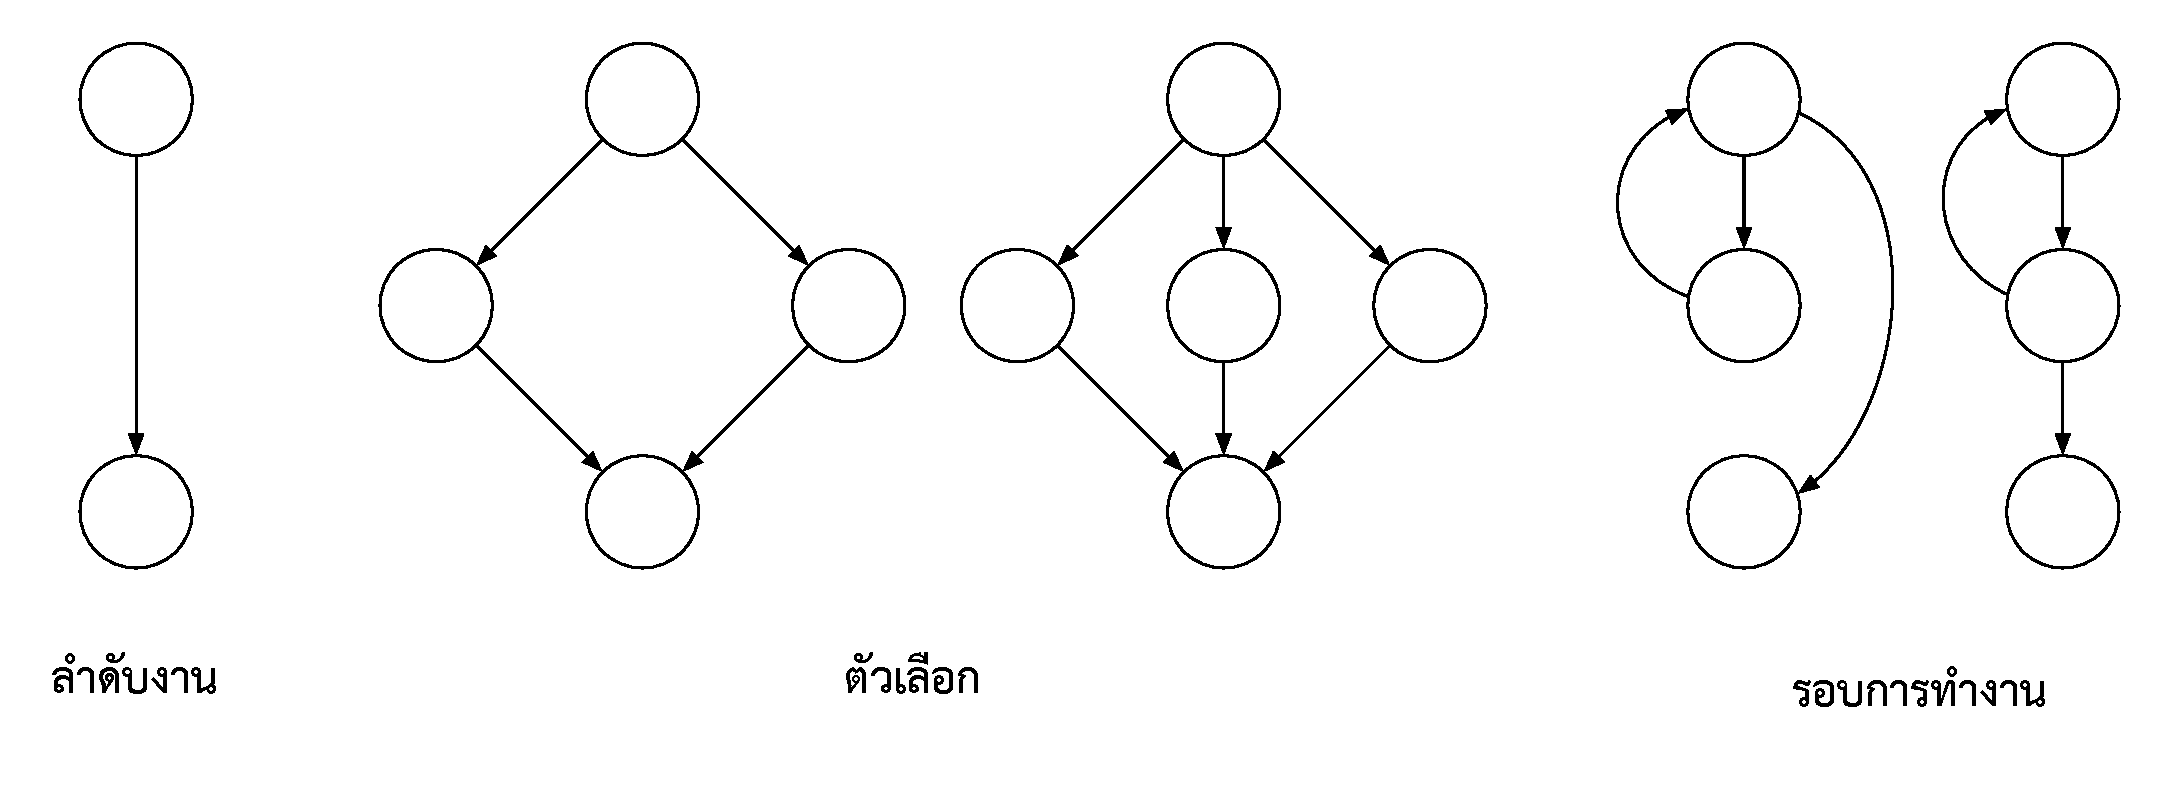
\includegraphics[width=0.9\textwidth]{graph-types}
    \caption{ประเภทของกราฟ}
    \label{fig:graphtype}
\end{figure}

จาก\figref{fig:pseudocodeGrading} เป็นชุดรหัสเทียมที่นำเสนอวิธีการคำนวณเกรดของนิสิตโดยรับข้อมูล โดยรับข้อมูลคะแนน (student\_score) 
และคะแนนพิเศษ (bonus\_score) ของนิสิต หากมีคะแนนเป็น 0 จะได้เกรด \emph{{\bf I}} หากนิสิตได้คะแนนต่ำกว่า 80 คะแนน 
จะได้เกรด {\emph{\bf U}} หากมีคะแนนตั้งแต่ 80 ไปจนถึง 100 คะแนน นิสิตจะได้เกรด {\emph{\bf S}} ซึ่งจากชุดรหัสเทียมนี้ 
สามารถแปลงเป็นกราฟโปรแกรม เพื่อทำความเข้าใจโครงสร้างได้ดัง{\figref{fig:programGraph} 

\begin{figure}[ht!]
    \begin{algorithm}[H]
        \begin{algorithmic}[1]
            \STATE{Program {\bf "Simple Grading"}}
            \STATE{student\_score $\gets$ receive student score}
            \STATE{bonus\_score $\gets$ receive student's bonus score}

            \IF{bonus\_score > 0}
                \IF{student\_score <= 50} 
                    \STATE{student\_score = min(50, student\_score + bonus\_score)} 
                \ELSIF{student\_score <= 70} 
                    \STATE{student\_score = min(70, student\_score + bonus\_score)}
                \ENDIF
            \ENDIF

            \STATE{grade\_letter = ""}

            \IF{student\_score < 80} 
                \STATE{grade\_letter = 'U'} 
            \ELSIF{student\_score == 0}
                \STATE{grade\_letter = 'I'} 
            \ELSIF{student\_score <= 100}
                \STATE{grade\_letter = 'S'} 
            \ENDIF

            \STATE{print(grade\_letter)}
        \end{algorithmic}
    \end{algorithm}
    \caption{ชุดรหัสเทียมสำหรับคำนวณเกรดนิสิตจากคะแนนที่ได้รับ}
    \label{fig:pseudocodeGrading}
\end{figure}


\begin{figure}[ht!]
    \centering
    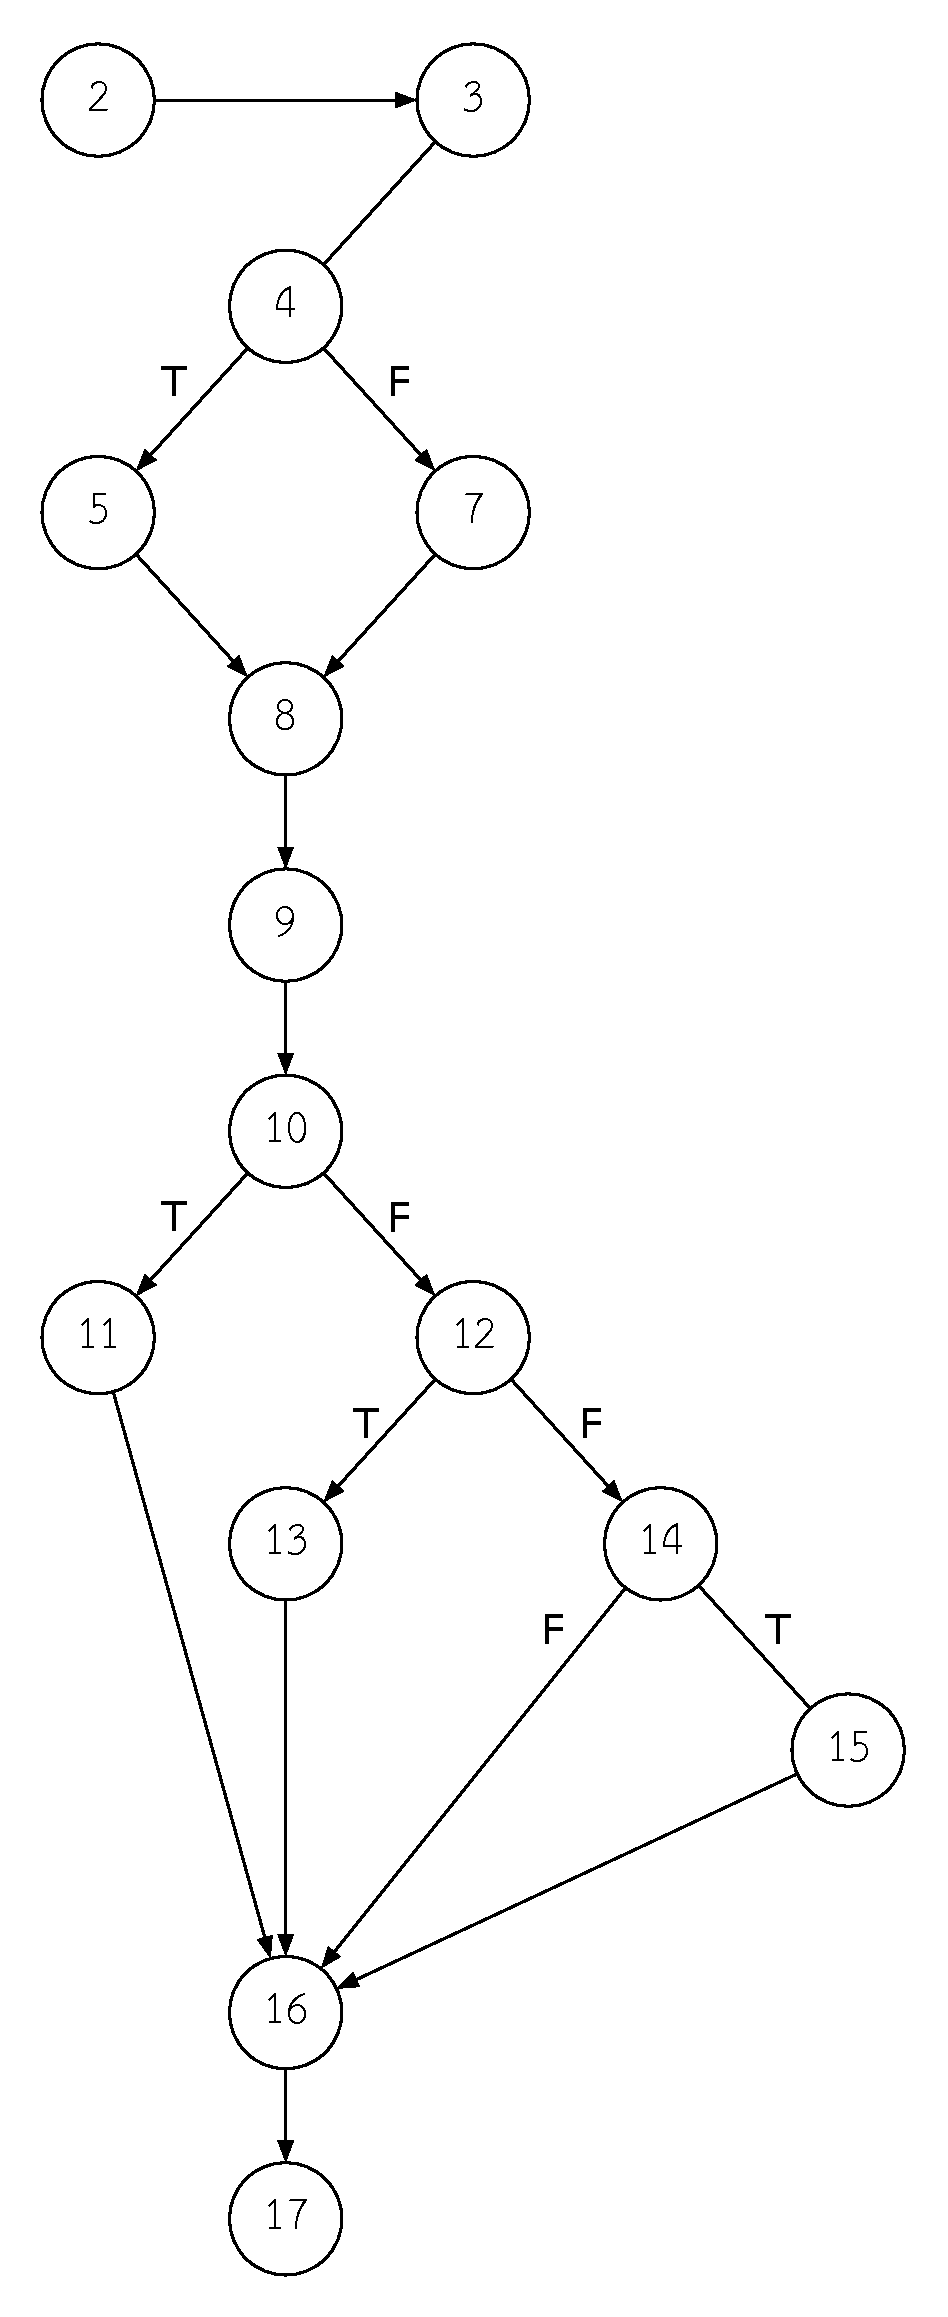
\includegraphics[height=0.80\textheight]{grading-program-graph}
    % - - - - - - - - - - - - - - - - - - - -
    % \begin{tikzpicture}[node distance=2cm]
    %     % Nodes layout
    %     \node[shape=circle,draw=black] (4) {$4$};
    %     \node[shape=circle,draw=black, above left of=4] (2) {$2$};
    %     \node[shape=circle,draw=black, above right of=4] (3) {$3$};
    %     \node[shape=circle,draw=black, below left of=4] (5) {$5$};
    %     \node[shape=circle,draw=black, below left of=5] (6) {$6$};
    %     \node[shape=circle,draw=black, below right of=5] (7) {$7$};
    %     \node[shape=circle,draw=black, below left of=7] (8) {$8$};
    %     \node[shape=circle,draw=black, below right of=8] (9) {$9$};
    %     \node[shape=circle,draw=black, below left of=9] (10) {$10$};
    %     \node[shape=circle,draw=black, below of=10] (11) {$11$};
    %     \node[shape=circle,draw=black, below of=11] (12) {$12$};
    %     \node[shape=circle,draw=black, below left of=12] (13) {$13$};
    %     \node[shape=circle,draw=black, below right of=13] (14) {$14$};
    %     \node[shape=circle,draw=black, below left of=14] (15) {$15$};
    %     \node[shape=circle,draw=black, below right of=14] (16) {$16$};
    %     \node[shape=circle,draw=black, below left of=16] (17) {$17$};
    %     \node[shape=circle,draw=black, below of=17] (18) {$18$};
    %     \node[shape=circle,draw=black, below of=18] (19) {$19$};

    %     % Connected edges 
    %     % \path [->] (A) edge node[midway, above]{This works} (B);
    %     \path [->] (2) edge (3);
    %     \path [->] (3) edge node[midway, above]{T} (4);
    %     \path [->] (4) edge node[midway, above]{F} (10);

    %     \path [->] (4) edge node[midway, above]{T} (5);
    %     \path [->] (5) edge node[midway, above]{T} (6);
    %     \path [->] (5) edge node[midway, above]{F} (7);
    %     \path [->] (7) edge node[midway, above]{T} (8);
    %     \path [->] (8) edge node[midway, above]{F} (9);
    %     \path [->] (9) edge node[midway, above]{F} (10);
    %     \path [->] (10) edge (11);
    %     \path [->] (11) edge (12);
    %     % \path [->] (9) edge node[midway, above]{F} (10);

    % \end{tikzpicture}
    % - - - - - - - - - - - - - - - - - - - -
    \caption{กราฟโปรแกรมของชุดรหัสเทียมสำหรับคำนวณเกรดนิสิต}
    \label{fig:programGraph}
\end{figure}

จาก{\figref{fig:programGraph}} เป็นการนำเสนอชุดรหัสเทียมจาก{\figref{fig:pseudocodeGrading} ในรูปของกราฟโปรแกรม 
โดยที่{\Node}ที่ 2-3, 6, 8, 9, 10, 11, 13, 17, 18 และ 19 คือ{\Node}ที่แสดงถึงลำดับการดำเนินงาน 
และ{\Node} 4, 5, 6, 7, 12, 14 และ 16 เป็น{\FirstTimeDefine{\PredicateNode}{\PredicateNodeEN}} ภายในโปรแกรม 
โดยมีโหนด 2 และ 19 เป็น{\FirstTimeDefine{\sourcenode}{\sourcenodeEN}} 
และ{\FirstTimeDefine{\sinknode}{\sinknodeEN}}\ ตามลำดับ 

การนำเสนอโปรแกรมในรูปของกราฟโปรแกรมนั้นช่วยให้ผู้ทดสอบวิเคราะห์โครงสร้างของโปรแกรมจากกราฟ 
เพื่อหาข้อผิดพลาดในโครงสร้างของโปรแกรมง่ายขึ้น ด้วยการแยก{\FirstTimeDefine{\BasisPath}{\BasisPathEN}} 
จากกราฟข้างต้น โดยแต่ละ{\BasisPath}ที่แยกนั้นจะเริ่มต้นด้วย{\sourcenode} และสิ้นสุดด้วย{\sinknode}เดียวกัน ซึ่งในที่นี้คือ 2 และ 19
กำหนด{\BasisPath}ที่ต้องการทดสอบเป็น \FirstTimeDefine{\TestPath}{\TestPathEN} จากนั้นจึงวิเคราะห์{\PredicateNode}
ที่ปรากฎบน{\TestPath} พิจารณาเงื่อนไข แล้วจึงสร้างกรณีทดสอบพร้อมทั้งข้อมูลทดสอบตามวิธีการที่ผู้ทดสอบเห็นสมควร 
ซึ่งจะได้กรณีทดสอบที่ทำให้โปรแกรมดำเนินการบน{\TestPath} ที่เลือกมาได้ ยกตัวอย่างเช่น 
หากเลือก{\BasisPath}จาก{\figref{fig:programGraph}} เป็น{\TestPath} จะพบว่ามี{\PredicateNode}บน{\TestPath} 3 {\Node} 
ด้วยกัน นั่นคือ {\bf 4}, {\bf 5} และ {\bf 10} เมื่อพิจารณา{\PredicateNode}ทั้ง 3 {\Node}จะได้ข้อมูลทดสอบเป็น {\bf bonus\_score = 1} และ 
{\bf student\_score = 50} ซึ่งข้อมูลทดสอบที่สร้างขึ้นนี้สามารถทำให้โปรแกรมทำงานใน{\TestPath}ได้ 
ดังกรณีทดสอบใน\tabref{tab:simpleTestCase}

\clearpage
\begin{figure}[ht!]
    \centering
    \small{$2\ \textendash\ 3\ \textendash\ 
                (4)\ \textendash\ (5)\ \textendash\ 6\ \textendash\ 10\ \textendash\ 
                11\ \textendash\ (12)\ \textendash\ 13\ \textendash\ 18 \textendash\ 19$}
    \caption{ตัวอย่าง{\TestPath}สำหรับโปรแกรมคำนวณเกรด}
    \label{fig:testpath}
\end{figure}


\begin{table}[ht!]
    \centering
    \caption{กรณีทดสอบ}
    \label{tab:simpleTestCase}
    \begin{tabular}{|l|c|c|c|}
    \hline
    \rowcolor{LightGray}
    Case ID     & bonus\_score  & student\_score    & Expected output \\
    \hline
    SC1         & 1             & 50                & U \\
    \hline
    \end{tabular}
\end{table}

\subsection{\FirstTimeDefine{\scg}{\scgEN}}

% การพัฒนาโปรแกรมเชิงวัตถุ (Object-oriented programing: OOP) คือการจำลองพฤติกรรมและความสามารถจากชีวิตจริงออกมาเป็น
% {\FirstTimeDefine{\class}{\classEN}} \FirstTimeDefine{\method}{\methodEN} 
% และ{\FirstTimeDefine{\attribute}{\attributeEN}} \cite{kindler2011} ซึ่งโปรแกรมใด
% โปรแกรมหนึ่งที่พัฒนาขึ้นด้วยแนวคิดการพัฒนาเชิงวัตถุ นั่นคือการดำเนินงานสอดประสานร่วมกันของ{\class}ผ่าน{\method} 
% ดังนั้นเพื่อให้เข้าใจถึงความสัมพันธ์กันระหว่าง{\sourcecode} ด้วย{\scg} โดยที่แต่ละ{\Node}แทน{\class} 
% หากคลาสเรียกใช้งาน{\method}ของ{\class}อื่น ตัวอย่างเช่น หากแปลงชุดรหัสเทียมจาก \figref{fig:pseudocodeGrading} 
% เป็น{\sourcecode}ภาษาจาวา (Java) ตามแนวคิดเชิงวัตถุ 
% ด้วยแนวคิดพื้นฐานของออกแบบเชิงวัตถุ (Object-oriented design) \cite{Martin2016} นิยามไว้โดย Robert C. Martin 
% ซึ่งเป็นแนวคิดการออกแบบที่นักพัฒนานำไปใช้งานโดยทั่วไป 
การพัฒนาโปรแกรมเชิงวัตุ (Object-oriented programming: OOP) เป็นการรวมพฤติกรรม และความสามารถที่คล้ายคลึงกันเข้าไว้ด้วยกัน \cite{kindler2011}
เป็น\FirstTimeDefine{\class}{\classEN} \FirstTimeDefine{\method}{\methodEN} และ \FirstTimeDefine{\attribute}{\attributeEN} 
และเพื่อให้เข้าใจถึงการเกิดปฏิสัมพันธ์ซึ่งกันและกันระหว่าง{\class}ภายในซอฟต์แวร์ภายใต้การทดสอบ (Software under test: SUT) จาก{\sourcecode} 
ที่ได้รับมานั้น จึงจำเป็นจะต้องพิจารณา{\sourcecode}แล้วจึงนำมาสร้างเป็น \FirstTimeDefine{\scg}{\scgEN} โดยที่{\scg} 
นั้นจะใช้{\Node}แทน{\class}ทั้งหมด เชื่อมกันด้วย{\Edge}ที่กำกับด้วย{\method}ที่{\class}ใช้ปฏิสัมพันธ์กัน หากแปลง{\sourcecode}จาก
\figref{fig:pseudocodeGrading} ให้เป็น{\sourcecode}ภาษาจาวา (Java) โดยแยกออกเป็น 3 \class\ ได้แก่ \code{SimpleQuiz} 
ทำหน้าที่อ่านข้อมูลคำถามภายในชั้นเรียน \code{SimpleBonusScore} ทำหน้าที่คำนวณคะแนนเพิ่มพิเศษ และ \code{SimpleGrading} ทำหน้าที่คำนวณเกรดของนิสิต 
ดัง \figref{fig:javaQuiz} \figref{fig:javaBonusScore} และ\figref{fig:javaGrading}ตามลำดับ

\begin{figure}[ht!]
    \lstset{basicstyle=\small,style=thesiscodestyle,language=java}
    \lstinputlisting[language=Java]{related/SimpleQuiz.java}
    \caption{{\sourcecode}ภาษาจาวาสำหรับอ่านคะแนนคำถามภายในชั้นเรียน}
    \label{fig:javaQuiz}
\end{figure}

\begin{figure}[ht!]
    \lstset{basicstyle=\small,style=thesiscodestyle,language=java}
    \lstinputlisting[language=Java]{related/SimpleBonusScore.java}
    \caption{{\sourcecode}ภาษาจาวาสำหรับคำนวนคะแนนเพิ่มพิเศษ}
    \label{fig:javaBonusScore}
\end{figure}

\begin{figure}[ht!]
    \lstset{basicstyle=\small,style=thesiscodestyle}
    \lstinputlisting[language=Java]{related/SimpleGrading.java}
    \caption{{\sourcecode}ภาษาจาวาสำหรับคำนวณเกรดนิสิต}
    \label{fig:javaGrading}
\end{figure}

\clearpage
จาก\figref{fig:javaGrading} เมื่อกำหนดให้ \code{Q} แทน\class\ \code{SimpleQuiz}, \code{G} แทน{\class} \code{SimpleGrading} 
และ \code{B} แทน\class\ \code{SimpleBonusScore} โดยที่\class\ \code{SimpleGrading} เรียกใช้งาน{\method} \code{score} 
ซึ่งเป็น{\method}ของ{\class} \code{SimpleBonusScore} ผ่าน{\method} {\code{grading}} ดังนั้น{\scg}สำหรับความสัมพันธ์นี้จะเป็นดัง
{\figref{fig:scggrading}} ซึ่งในการพัฒนาจริงนั้น\class\ \code{SimpleGrading} และ\class\ \code{SimpleBonusScore}
อาจมีการเรียกใช้งานระหว่างกันมากกว่า 1 \method % ดังที่ได้แสดงใน{\figref{fig:subactualscg}}

\begin{figure}[htb!]
    \centering
    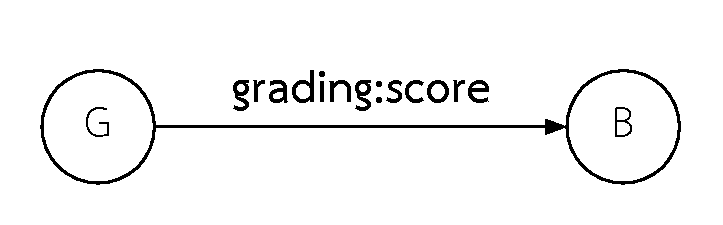
\includegraphics[width=0.8\textwidth]{simple-static-call-graph}
    % \begin{minipage}[t]{0.5\linewidth}
    %     \centering
    %     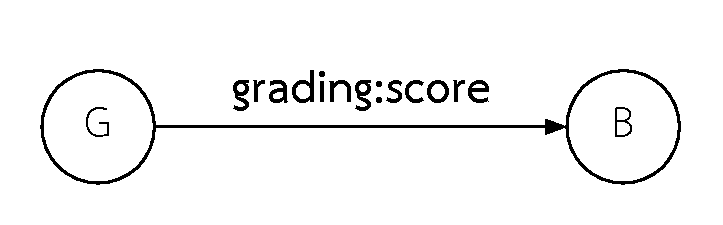
\includegraphics[width=0.8\textwidth]{simple-static-call-graph}
    %     \subcaption{{\scg}โปรแกรมคำนวณเกรดนิสิต}
    %     \label{fig:subscggrading}
    % \end{minipage}%
    % \begin{minipage}[t]{0.5\linewidth}
    %     \centering
    %     \includegraphics[width=0.8\textwidth]{simple-static-call-graph-multiple-call}
    %     \subcaption{{\scg}ของโปรแกรมในกรณีที่\code{SimpleGrading} มีการเรียกใช้งาน{\code{SimpleBonusScore}} หลาย{\method}}
    %     \label{fig:subactualscg}
    % \end{minipage}%
    \caption{{\scg}โปรแกรมคำนวณเกรดนิสิต}
    \label{fig:scggrading}
\end{figure}

% - - - - - - - - - - - - - - - - - - - -
\subsection{\FirstTimeDefine{\InfeasiblePath}{\InfeasiblePathEN}}

\InfeasiblePath คือ ทางเดินที่ไม่สามารถหาค่าทุก ๆ ความเป็นไปได้ซึ่งสอดคล้องกับ{\PredicateNode}ที่อยู่บนทางเดินนั้น 
เพื่อทำให้โปรแกรมทำงานบนเส้นทางนั้นได้ \cite{Naik2008} หากพิจารณาจากชุดรหัสเทียมใน{\figref{fig:pseudocodeGrading}} 
และกราฟใน{\figref{fig:programGraph}} ประกอบเข้าด้วยกัน จะพบว่าทางเดิน 
\code{\overline{12}\ \textendash\ 14\ \textendash\ 15 \textendash\ 18 \textendash\ 19} คือ {\bf \InfeasiblePath} 
ดังแสดงใน{\figref{fig:infeasiblePath}} เนื่องจากไม่สามารถหาค่าที่สอดคล้อง กับ\PredicateNode\ 12 และ 14 
นั่นคือ \code{student\_score \geq 80} และ \code{student\_score = 0} ได้ในทุก ๆ กรณี

\begin{figure}[t!]
    \centering
    \includegraphics[width=0.5\textwidth]{grading-program-graph-subgraph}
    \caption{โครงสร้างของโปรแกรมที่พบ{\InfeasiblePath}}
    \label{fig:infeasiblePath}
\end{figure}


ดังนั้นการทดสอบโปรแกรมนั้นจึงจำเป็นจะต้องวิเคราะห์{\InfeasiblePath}ที่อยู่ภายในโครงสร้างของโปรแกรมเพื่อรายงานผลให้นักพัฒนาได้ทราบและแก้ไข
ต่อไปได้

\subsection{\FirstTimeDefine{\Cyclomatic}{\CyclomaticEN}}

% การวัดความซับซ้อนของโปรแกรมนั้นสามารถทำได้หลายแนวทาง ทั้งการประมาณการจากจำนวนกรณีทดสอบ 
% ที่ครอบคลุม{\sourcecode}ได้ตามระดับความครอบคลุม (Coverage level) \cite{Ferrer2013} ตามที่ต้องการ
% หรือประเมินความซับซ้อนของแผนภาพกระบวนการทางธุรกิจ (Business Process Model and Notation: BPMN) ที่จะนำโปรแกรมเข้าไปช่วยบริหารจัดการ
% \cite{Solichah2013}
ในการวัดความซับซ้อนเชิงโครงสร้างของโปรแกรมนั้น McCabe ได้กำหนด \Cyclomatic\ \cite{McCabe1976}\ 
ไว้เพื่อเป็นมาตรวัดความซับซ้อนของโปรแกรม โดยใช้การพิจารณาจากจำนวน\Node\ \Edge และ\PredicateNode\ ที่ประกอบกันภายใน\ProgramGraph\ 
ดัง\eq{eq:complexitymeasureStronglyConnected} และ \eq{eq:complexitymeasure}

\begin{align}
    v(G) &= e - n + p \label{eq:complexitymeasureStronglyConnected} \\
    v(G) &= e - n + 2p \label{eq:complexitymeasure} 
\end{align}

\begin{table}[ht!]
    \begin{tabular}{lcl}
    เมื่อ & $v(G)$    & คือ ค่า{\Cyclomatic}ที่คำนวณได้               \\
        & $e$       & คือ จำนวน{\Edge}ใน\ProgramGraph            \\
        & $n$       & คือ จำนวน{\Node}ใน\ProgramGraph            \\
        & $p$       & คือ จำนวนพื้นที่ที่เชื่อมต่อกันใน\ProgramGraph   \\
    \end{tabular}
\end{table}

โดยที่ \eq{eq:complexitymeasureStronglyConnected} จะใช้กับกราฟที่เชื่อมต่อกันแบบเข้ม (Strongly connected graph) 
นั่นคือกราฟนั้นจะต้องมีทางเดินจาก $n_j$ ไปยัง $n_k$ เสมอ แต่หากไม่ใช่แล้วจะใช้ \eq{eq:complexitymeasure} โดยจะกำหนดให้ 
$p = 1$ จาก{\ProgramGraph}ใน{\figref{fig:programGraph}} ซึ่งมี{\Edge}ทั้งสิ้น 23 เส้น และจำนวน{\Node}ทั้งสิ้น 
18 \Node\ ดังนั้นหากคำนวนระดับความซับซ้อนตาม{\Cyclomatic}ของ{\ProgramGraph}นี้ จะได้ว่า

\begin{align*}
    v(G) &= e - n + 2p \\
         &= 23 - 18 + 2 \\
    v(G) &= 7 
\end{align*}

จากคำของ McCabe แล้วโปรแกรมไม่ควรมีค่า{\Cyclomatic}มากกว่า 15 โดยที่ค่าความซับซ้อนที่แนะนำอยู่ที่ 10 \cite{McCabe1976}


% \subsection{Feasible and Infeasible path}

วิธีการที่ใช้ในกระบวนการทดสอบซอฟต์แวร์

{\FeasiblePath}ใน{\sourcecode}


% \input{related/java-specification}

\subsection{การสร้างกรณีทดสอบอัตโนมัติ (Automated test case generation)}
\label{sub:tcgen}

% - อ้างอิงจาก "An orchestrated survey of methodologies for automated software test case generation" \cite{Anand2013} Part II
กระบวนการทดสอบซอฟต์แวร์นั้นสามารถสร้างกรณีทดสอบอัตโนมัติ ซึ่ง Anand และคณะ \cite{Anand2013} ได้แบ่งวิธีการสร้างกรณีทดสอบแบบอัตโนมัติไว้ทั้งหมด 
4 กลุ่มวิธีการด้วยกัน ซึ่งมี 2 กลุ่มวิธีการที่เกี่ยวข้องได้แก่

\subsubsection{Symbolic execution}
\label{sub:tcgen:sub:symbolic}

วิธีการนี้เป็นกระบวนการสร้างกรณีทดสอบที่ใช้การวิเคราะห์ชุดคำสั่งควบคุมการไหลของโปรแกรมแล้วสร้างเป็นเงื่อนไขของทางเดิน 
ใช้วิเคราะห์หาข้อมูลที่สามารถทำให้กรณีทดสอบนั้นสามารถทดสอบทางเดินที่เลือกได้ ซึ่งวิธีนี้มีประสิทธิภาพเรื่องความครอบคลุมของ{\sourcecode}ได้เป็นอย่างดี
หากแต่มีข้อเสียที่พบคือ โปรแกรมที่ใช้งานจริงนั้นมักจะมีเงื่อนไขหลากหลายและซับซ้อนเกินกว่าจะสร้างข้อมูลทดสอบอย่างอัตโนมัติได้ทั้งหมด 
นอกจากนั้นยังจำเป็นจะต้องอาศัยการตัดสินใจจากผู้ใช้งานในบางกรณี

\subsubsection{Random testing}
\label{sub:tcgen:sub:random}

จากศึกษาพบว่าข้อมูลที่ทำให้เกิดข้อผิดพลาดนั้นมีแนวโน้มที่จะอยู่รวมกันเป็นรูปแบบ %ดัง{\figref{fig:failureRegionPattern}} 
ดังนั้นกรณีทดสอบที่สร้างขึ้นควรจะต้องกระจายให้ครอบคลุมทั้งกลุ่มข้อมูลนำเข้า (Input domain) เพิ่มโอกาสการค้นหาข้อผิดพลาดภายในโปรแกรม 
ซึ่งมีแนวทาง Adaptive Random Testing โดย Chan และคณะ \cite{Chan2004}\ ที่พัฒนาขึ้นเพื่อเพิ่มประสิทธิภาพของ Random testing ในรูปแบบเดิม 
หากแต่ปัญหาของการทำ Random testing นั้นก็เกิดมาจากการต้องการสุ่มค่านั้นเอง 
เพราะมีโอกาสที่ค่าที่สุ่มขึ้นมานั้นมีจำนวนมาและไม่สามารถค้นพบข้อผิดพลาดที่อยู่ภายในโปรแกรมเลย ดังนั้นวิธีการหนึ่งที่มักจะอ้างถึงใน Adaptive Random Testing 
นั้นก็คือการกำหนดกลุ่มข้อมูลที่เป็นไปได้ (Fixed-Sized-Candidate-Set: FSCS-ART) ของ Adaptive Random Testing 
ด้วยการกำหนดค่าสูงสุดหรือต่ำสุดที่ต้องการสุ่มค่าออกมากได้ กำหนดรูปแบบหรือประเภทของข้อมูลที่ต้องการสุ่ม 
เพื่อให้ค่าที่สุ่มขึ้นมานั้นมีโอกาสในการค้นพบข้อผิดพลาดมากขึ้น % ใกล้เคียงกับความต้องการมากที่สุด


\subsection{การสร้างข้อมูลทดสอบ (Test data generation)}

- อธิบายการสร้างข้อมูลทดสอบที่ใช้งานกันอยู่ โดยอ้างจาก "An orchestrated survey of methodologies for automated software test case generation" \cite{Anand2013} - ส่วนที่ 2

\subsubsection{การสร้างข้อมูลทดสอบโดยใช้แบบจำลอง (Test data gerneration in model-based testing)}

- Overview กระบวนการ

- การทำงานตาม Paper: Modelling notations และเครื่องมือ

\subsubsection{Test data generation in combinatorial testing}

- วิธีการทั่วไปของ Combinatorial testing 

- ตัวอย่างการทดสอบสร้างข้อมูล

\subsubsection{การสร้างกรณีทดสอบด้วยการประยุกต์ใช้การสุ่มทดสอบ (Test data generation by adaptive random testing)}

- วิธีการ Random testing 

- การประยุกต์ใช้

- ประสิทธิภาพ

- ประสิทธิผล

- วิธีการที่นำไปใช้งาน



    \section{งานวิจัยที่เกี่ยวข้อง} 

\subsubsection{A Static Approach to Prioritizing JUnit Test Cases \cite{6363461}}
ที่มา

\subsubsection{Eclat: Automatic Generation and Classification of Test Inputs \cite{Heaton2000}}

\subsubsection{GRT: Program-analysis-guided random testing \cite{Ma2016}}
วิธีการสร้างกรอบข้อมูล เพื่อช่วยให้การสร้างข้อมูลทดสอบทำได้ง่ายมากยิ่งขึ้น

\subsubsection{Automatic generation and classification of test inputs \cite{Pacheco2005}}
การสร้างกลุ่มของกรณีทดสอบอย่างอัตโนมัติ ช่วยในการสร้างกรณีทดสอบ


    \section{แนวคิดและวิธีการดำเนินงาน}
\label{sec:methodology}

งานวิจัยนี้นำเสนอวิธีการสร้างกรณีทดสอบและข้อมูลทดสอบสำหรับ{\TestPath}ที่ครอบคลุมความสัมพันธ์ระหว่าง{\softwareComponent}ในรูปขอบ{\scg} 
ซึ่งได้จากการวิเคราะห์{\StaticInformation}ของ{\sourcecode}ภาษาจาวา แล้วจึงนำมาสร้างกรณีทดสอบตลอดจนข้อมูลทดสอบซึ่งสอดคล้องกับเงื่อนไขที่พบ
ดัง\figref{fig:methodologyoverview} ซึ่งมีแนวทางการดำเนินงานดังนี้

\begin{sidewaysfigure}
    \centering
    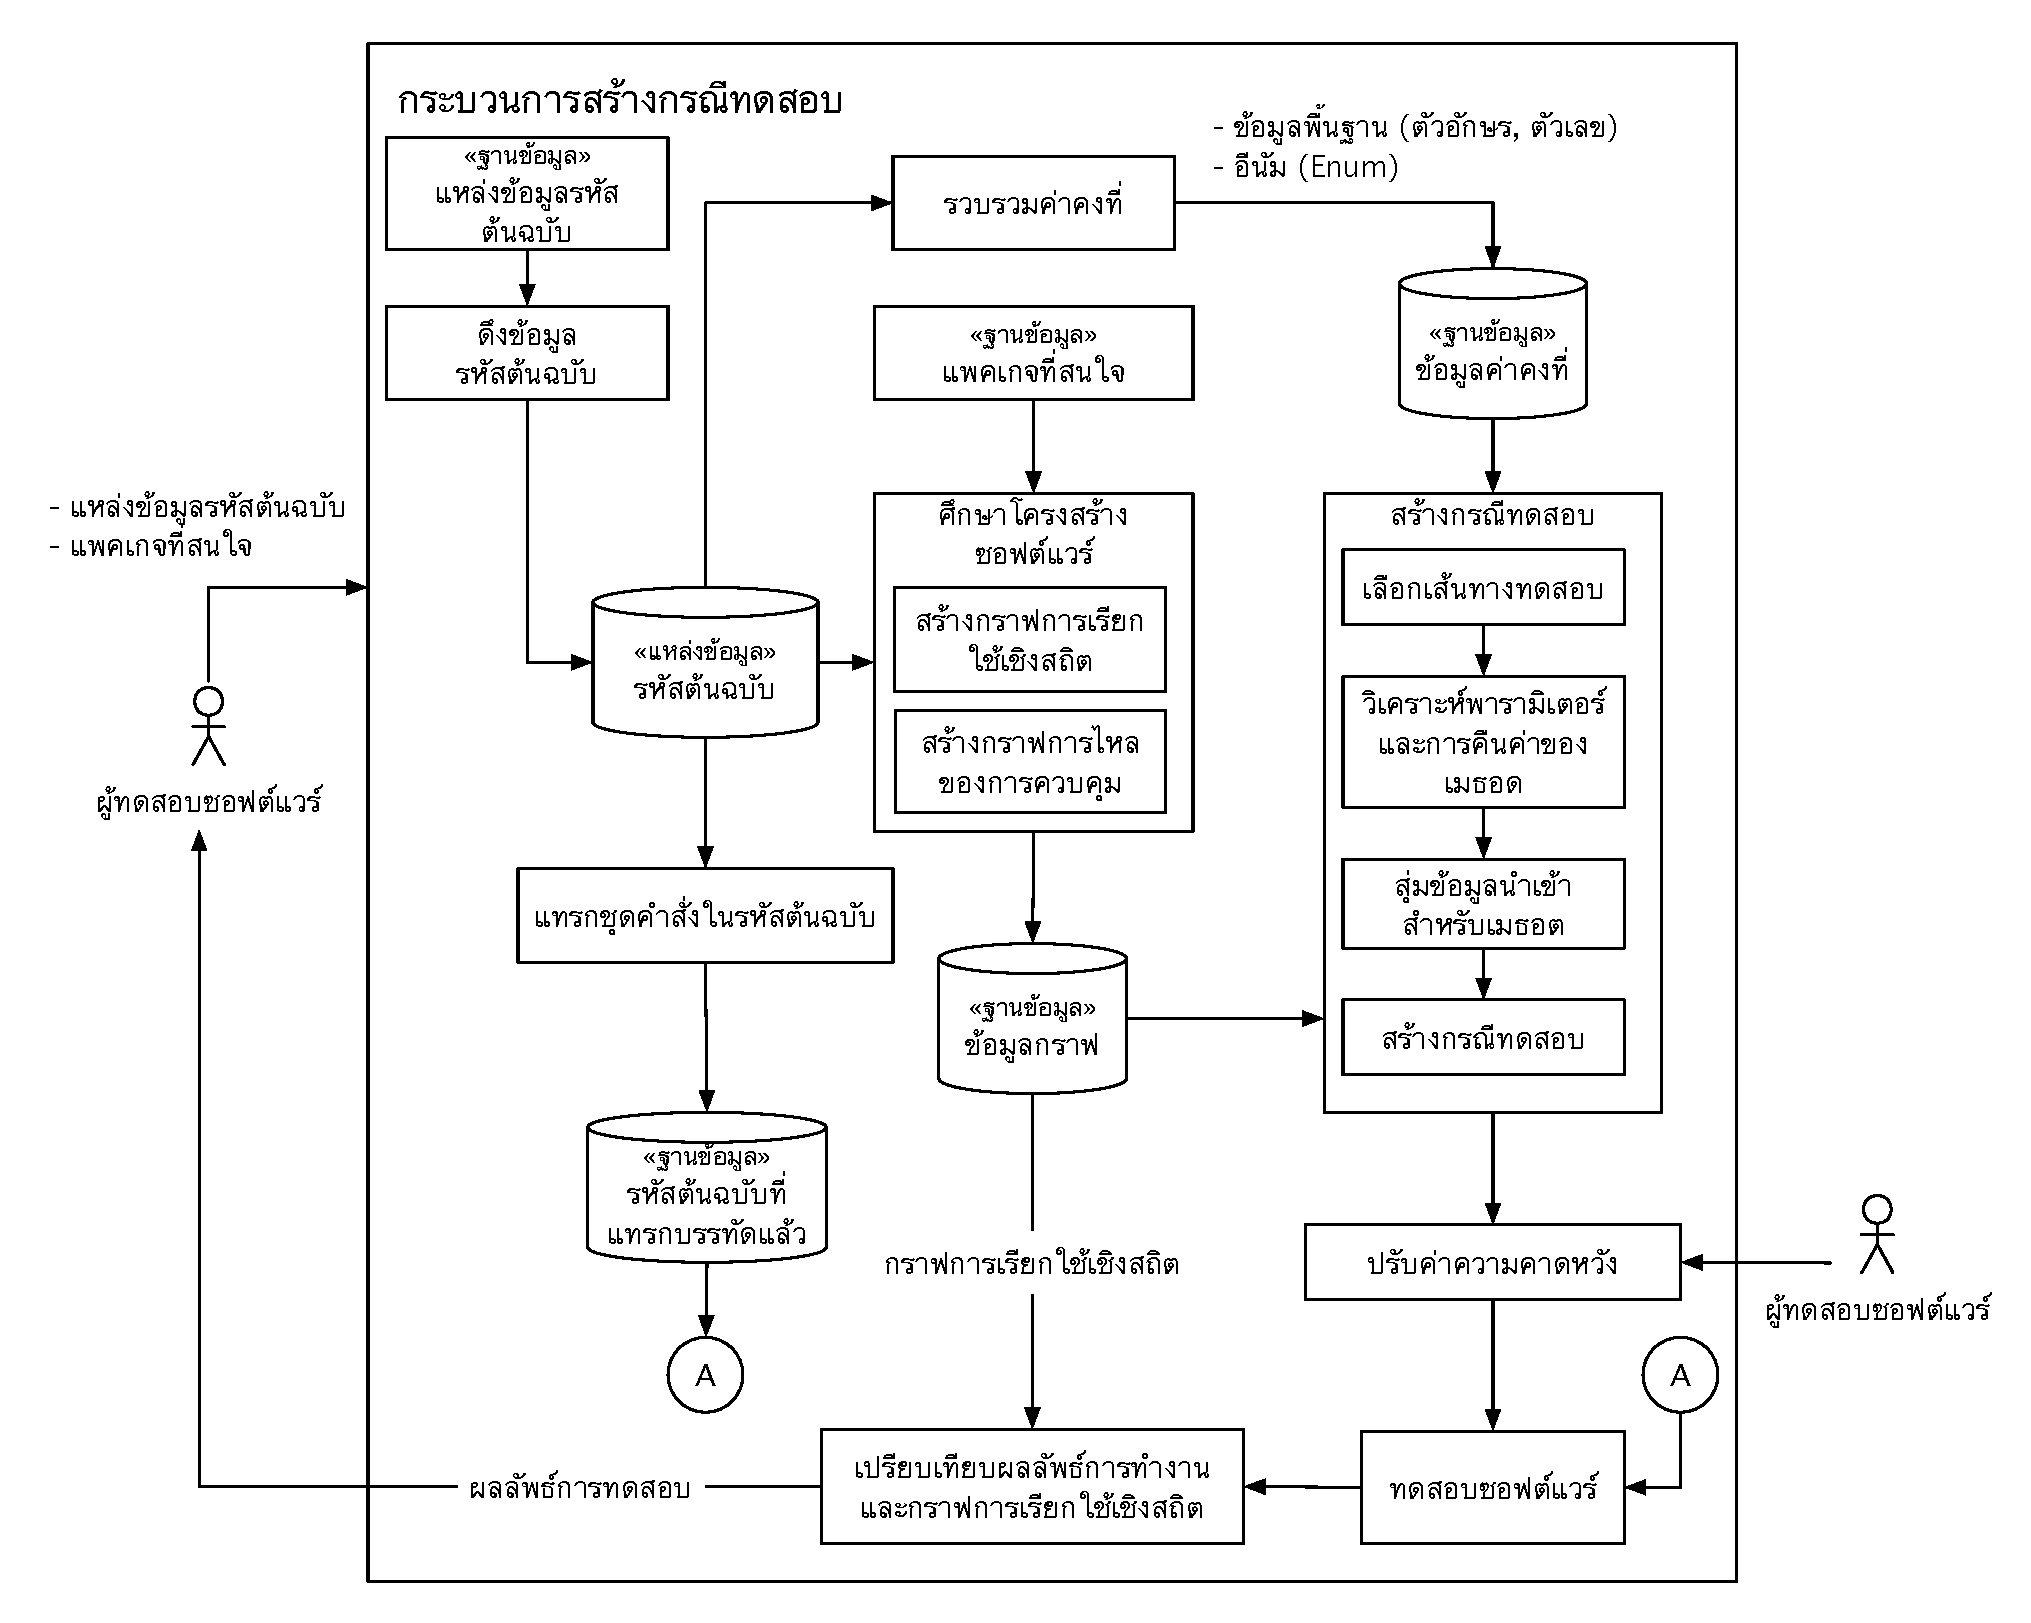
\includegraphics[width=0.9\textwidth]{methodology-overview}
    \caption{ภาพรวมการดำเนินงานวิจัย}
    \label{fig:methodologyoverview}
\end{sidewaysfigure}

\subsection{การวิเคราะห์ข้อมูลเบื้องต้น}
\label{subs:introsection}

ในขั้นตอนนี้เริ่มต้นด้วยการนำเข้าข้อมูล{\sourcecode}จาก{\Repository} เพื่อนำมารวบรวม{\StaticInformation} 
โดยสนใจเพียงเฉพาะ{\class}ซึ่งบรรจุอยู่ภายใน\FirstTimeDefine{\Package}{\PackageEN} ตามที่ผู้ใช้งานระบุ 
โดยกำหนดให้เป็น "\FirstTimeDefine{\CUT}{\CUTEN}" ทั้งนี้กระบวนการจะประกอบไปด้วย 3 ขั้นตอนด้วยกัน นั่นคือ
\FirstTimeDefine{\constantExtracting}, \FirstTimeDefine{\graphCreation}{\graphCreationEN} 
และ\FirstTimeDefine{\sourcecodeInstrumention}{\sourcecodeInstrumentionEN} 
โดยมีแนวทางการดำเนินงานของแต่ละขั้นตอน ดังนี้

\subsubsection{\FirstTimeDefine{\constantExtracting}{\constantExtractingEN}}
\label{sec:sub:sub:sourceCodeExtract}

การทำเหมืองข้อมูลค่าคงที่นั้นเป็นกระบวนการเพื่อกำหนดแนวทางการในการสร้างข้อมูลทดสอบสำหรับ{\TestPath}ที่เลือก โดยมีแนวทางการจัดเก็บค่าคงที่ที่ประกาศไว้
ภายใน{\sourcecode} โดยสนใจกลุ่มข้อมูล 2 กลุ่ม ได้แก่

\begin{enumerate}
    \item {\it ข้อมูลพื้นฐาน (Primitive data)} ซึ่งเป็นข้อมูลพื้นฐานที่ใช้งานภายใน{\class} ซึ่งในที่นี้จะสนใจข้อมูลพื้นฐาน 2 ประเภทได้แก่
        \begin{enumerate}
            \item {\bf ตัวอักษร} ซึ่งมีประเภทข้อมูลเป็น \code{String} ในภาษาจาวา
            \item {\bf ตัวเลข} ซึ่งมีประเภทข้อมูล ได้แก่ \code{byte, short, int, long, float} และ\code{double} ในภาษาจาวา
        \end{enumerate}
    \item {\it โครงสร้างข้อมูลจำกัดเขต (Enumeration)} ซึ่งมีประเภทข้อมูลเป็น \code{enum} ในภาษาจาวา
\end{enumerate}

ทั้งนี้จะไม่สนใจข้อมูลเชิงตรรกะ (มีชนิดข้อมูลเป็น \code{bool} ในภาษาจาวา) เนื่องมาจากว่าตัวเลือกที่เป็นไปได้จำกัดอยู่แล้ว 
นอกจากนั้นจะยังไม่สนใจข้อมูลจำเพาะ ที่กำหนดขึ้นมาใช้งานเอง 
จาก{\sourcecode}ของ{\class} \code{SimpleBonusScore} และ\code{SimpleGrading} ดังที่แสดงใน 
\figref{fig:javaBonusScore} และ \ref{fig:javaGrading} ตามลำดับ ในการดำเนินการวิจัยครั้งนี้ 
จะจัดเก็บข้อมูลค่าคงที่ซึ่งอยู่ในบรรทัดที่ \code{6, 8, 9, 10, 11, 12, 15, 16, 17} และ \code{18} ของ{\class} \code{SimpleBonusScore}
ตลอดจนค่าคงที่ซึ่งอยู่ในบรรทัดที่ \code{4, 5, 6, 8, 9} และ \code{10} ของ{\class} \code{SimpleGrading} 
แล้วจึงนำมาจัดเก็บไว้ภายในฐานข้อมูลโดยแยกตาม{\class}ที่พบค่าคงที่เหล่านั้น เพื่อใช้ในขั้นตอน {\bf \testcaseGeneration} ต่อไป

หลังจากรวบรวม{\bf ค่าคงที่}จาก{\sourcecode}ได้เรียบร้อยแล้ว จะนำ{\bf ข้อมูลพื้นฐาน} และ{\bf โครงสร้างข้อมูลจำกัดเขต} ที่รวบรวมได้
จัดหมวดหมู่และบันทึกไว้ภายใน{\it ฐานข้อมูล}

\subsubsection{\FirstTimeDefine{\graphCreation}{\graphCreationEN}}
\label{sec:sub:sub:graphCreation}

กระบวนการสร้างกราฟนั้นจะรับข้อมูล{\sourcecode}จาก{\Repository}เพื่อนำข้อมูลมาใช้สร้างกราฟ โดยแบ่งออกเป็น 2 กระบวนการย่อยด้วยกัน 
นั้นคือ การสร้าง{\scg} และการสร้าง{\cfg} ดังนี้

\begin{enumerate}
    \item {\bf สร้าง{\scg}} อ่านข้อมูล{\CUT}ตามที่ผู้ใช้งานสนใจ แล้วนำมาสร้าง{\scg} โดยผลลัพธ์ที่ได้นั้นจะแบ่งเป็น 3 กลุ่ม ได้แก่
        \begin{enumerate}
            \item การเรียกใช้งานระหว่าง{\CUT}ด้วยกัน \label{ord:scgcut} 
            \item การเรียกใช้งานระหว่าง{\CUT}และ{\class}ภายในชุดพัฒนาของจาวา (Java SDK) \label{ord:scgjdk} 
            \item การเรียกใช้งานระหว่าง{\CUT}และชุดคำสั่งภายนอก (\code{3^{rd}} party library) \label{ord:scg3rd} 
        \end{enumerate}
        ซึ่งในแนวทางการดำเนินงานนี้จะสนใจเฉพาะ{\scg}ของ{\CUT}เท่านั้น ดังนั้นในขั้นตอนนี้ไม่สนใจกราฟที่เกิดจากการเรียกใช้ในข้อ 1.2
        และ 1.3 ตลอดจนกราฟที่เกิดจากการสร้างวัตถุใหม่ เพื่อให้ได้{\scg}เฉพาะ{\CUT} ดังเช่น{\scg}โปรแกรมคํานวณเกรดนิสิต ใน\figref{fig:scggrading}

    \item {\bf สร้าง{\cfg}} โดยจะอ่านข้อมูลของ{\CUT}นำมาสร้าง{\cfg}และจัดเก็บข้อมูลไว้ภายในฐานข้อมูล
\end{enumerate}

เมื่อสิ้นสุดกระบวนการจะนำข้อมูล{\bf {\scg}} และ{\bf {\cfg}} ที่ได้จัดเก็บลง {\it ฐานข้อมูล} เพื่อจัดเตรียมไว้สำหรับ 
{\bf ขั้นตอนการสร้างกรณีทดสอบ} และ{\bf เปรียบเทียบผลลัพธ์การดำเนินการ} ต่อไป

\subsubsection{\FirstTimeDefine{\sourcecodeInstrumention}{\sourcecodeInstrumentionEN}}
\label{sec:sub:sub:srcInstrument}

เนื่องจากว่าการทดสอบนี้จำเป็นต้องครอบคลุม{\Path}ระหว่าง{\CUT} ดังนั้นจำเป็นจะต้องแทรกชุดคำสั่งใน{\sourcecode}ในแต่ละขั้นตอนการทำงาน 
จากนั้นจึงนำ{\sourcecode}ที่ผ่านการแทรกชุดคำสั่งเรียบร้อยแล้วไปใช้ในกระบวนการทดสอบ 
แล้วจึงจัดเก็บผลลัพธ์ที่ได้ระหว่างขั้นตอนการทดสอบ เพื่อนำมาเปรียบเทียบกับ{\TestPath}ที่เลือก

\begin{figure}[hbt!]
    \lstset{style=thesiscodestyle}
    \lstinputlisting[language=java]{methodology/SimpleBonusScoreInstrumented.java}
    \caption{{\class} \code{SimpleBonusScoreInstrumented}}
    \label{fig:javaBonusScoreInstrumented}
\end{figure}

จากตัวอย่าง\figref{fig:javaBonusScoreInstrumented} เป็น{\sourcecode}ที่สืบเนื่องมาจาก\figref{fig:javaBonusScore}
แต่ต่างกันโดยแทรกชุดคำสั่งเข้าไปภายใน{\sourcecode} ณ บรรทัดที่ \code{3, 6, 8, 11, 16, 19} และ \code{25} ซึ่งการแทรกชุดคำสั่งในกระบวนการนี้จะสนใจเพียงแค่{\CUT} เท่านั้น

เมื่อเสร็จสิ้นกระบวนการแทรกชุดคำสั่ง จะนำ{\sourcecode}ที่ได้จัดเก็บไว้ใน {\it ฐานข้อมูล} เพื่อจัดเตรียมไว้สำหรับนำไปทดสอบอีกครั้ง

\clearpage
\subsection{\FirstTimeDefine{\testcaseGeneration}{\testcaseGenerationEN}}
\label{sec:sub:tcg}

การดำเนินงานวิจัยในครั้งนี้จะนำ {\bf ข้อมูลกราฟ} ซึ่งประกอบไปด้วย {\it {\scg}} ร่วมกับ{\it {\cfg}} ใช้เป็นข้อมูลเริ่มต้นเพื่อสร้าง{\TestPath}
ระหว่าง{\CUT} ให้ครอบคลุมความสัมพันธ์ระหว่าง{\class} ดังที่ปรากฎใน{\scg} โดยจะสร้างกรณีทดสอบโดยพิจารณาจาก{\PredicateNode}ที่ปรากฎบน{\TestPath}ที่เลือก 
สุดท้ายจึงนำข้อมูลทั้งหมดที่ได้สร้างเป็นชุดกรณีทดสอบ โดยมีภาพรวมการดำเนินงานดัง \figref{fig:testcaseGenerationActivity}

\begin{figure}[ht!]
    \centering
    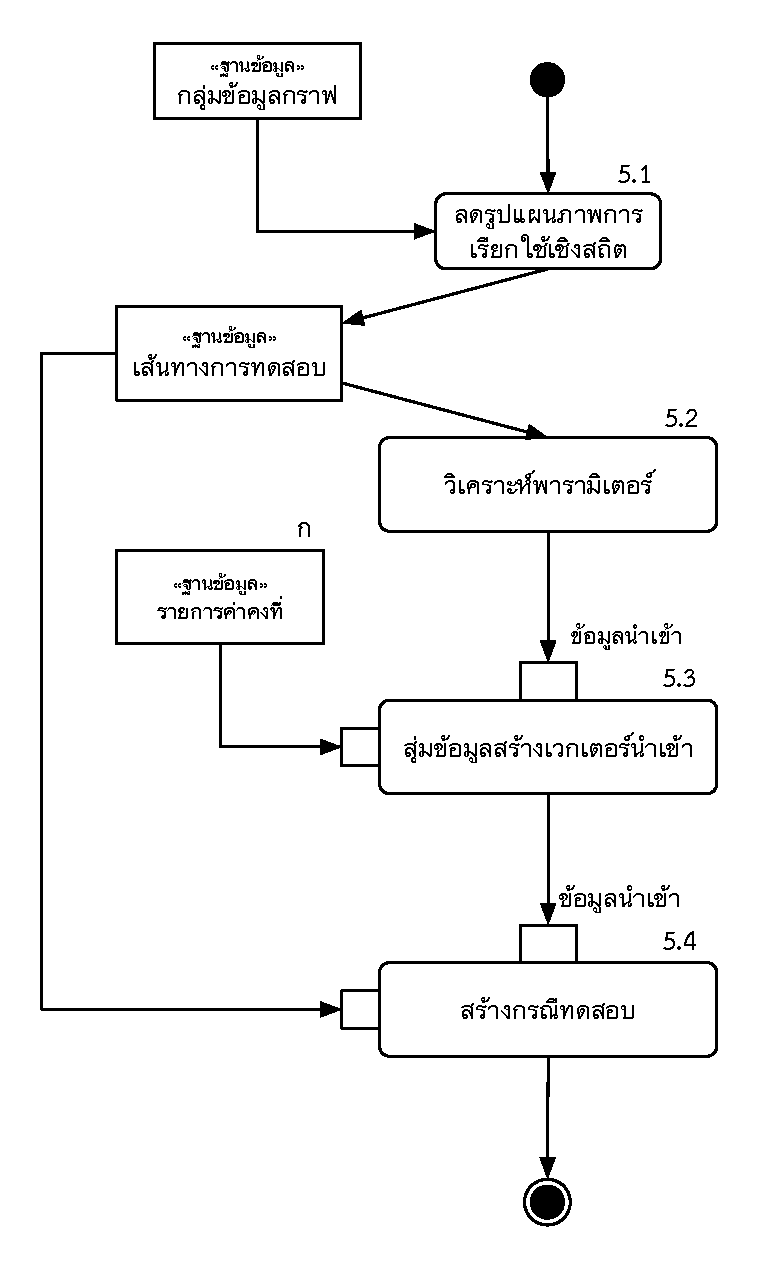
\includegraphics[width=0.5\textwidth]{methodology-activities-test-case-gen}
    \caption{ขั้นตอนการสร้างกรณีทดสอบ}
    \label{fig:testcaseGenerationActivity}
\end{figure}

\subsubsection{\FirstTimeDefine{\testpathSelection}{\testpathSelectionEN}}

ในขั้นตอนนี้จะพิจารณาจากข้อมูล{\it \scg} ร่วมกับ {\it \cfg} เพื่อเลือก{\TestPath}ที่ครอบคลุมความสัมพันธ์ระหว่าง{\class}ที่ปรากฎบน{\scg} 
เฉพาะระหว่าง{\CUT} ซึ่งจาก{\scg}ตัวอย่างใน\figref{fig:scggrading} จะได้{\TestPath} 2 {\Path} ด้วยกันคือ

\begin{enumerate}
    \item[\code{P_1:}] \code{G - [grading:score] - B - [score:getQuizScore] - Q}
    \item[\code{P_2:}] \code{G - [grading:score] - B - [score:getQuizSum] - Q}
\end{enumerate}

เพื่อให้ทราบถึงเงื่อนไขที่ทำให้กรณีทดสอบที่สร้างขึ้นสามารถทดสอบ{\TestPath}ข้างต้นได้ จึงใช้{\cfg}ของ{\method} \code{grading} จาก{\class} \code{SimpleGrading}, 
{\method} \code{score} จาก{\class} \code{SimpleBonusScore} รวมทั้ง{\method} \code{getQuizeScore} และ \code{getQuizSum} จาก{\class} \code{SimpleQuiz}
รวมพิจารณา ดัง\figref{fig:callreferences}

\begin{sidewaysfigure}[hbt!]
    \centering
    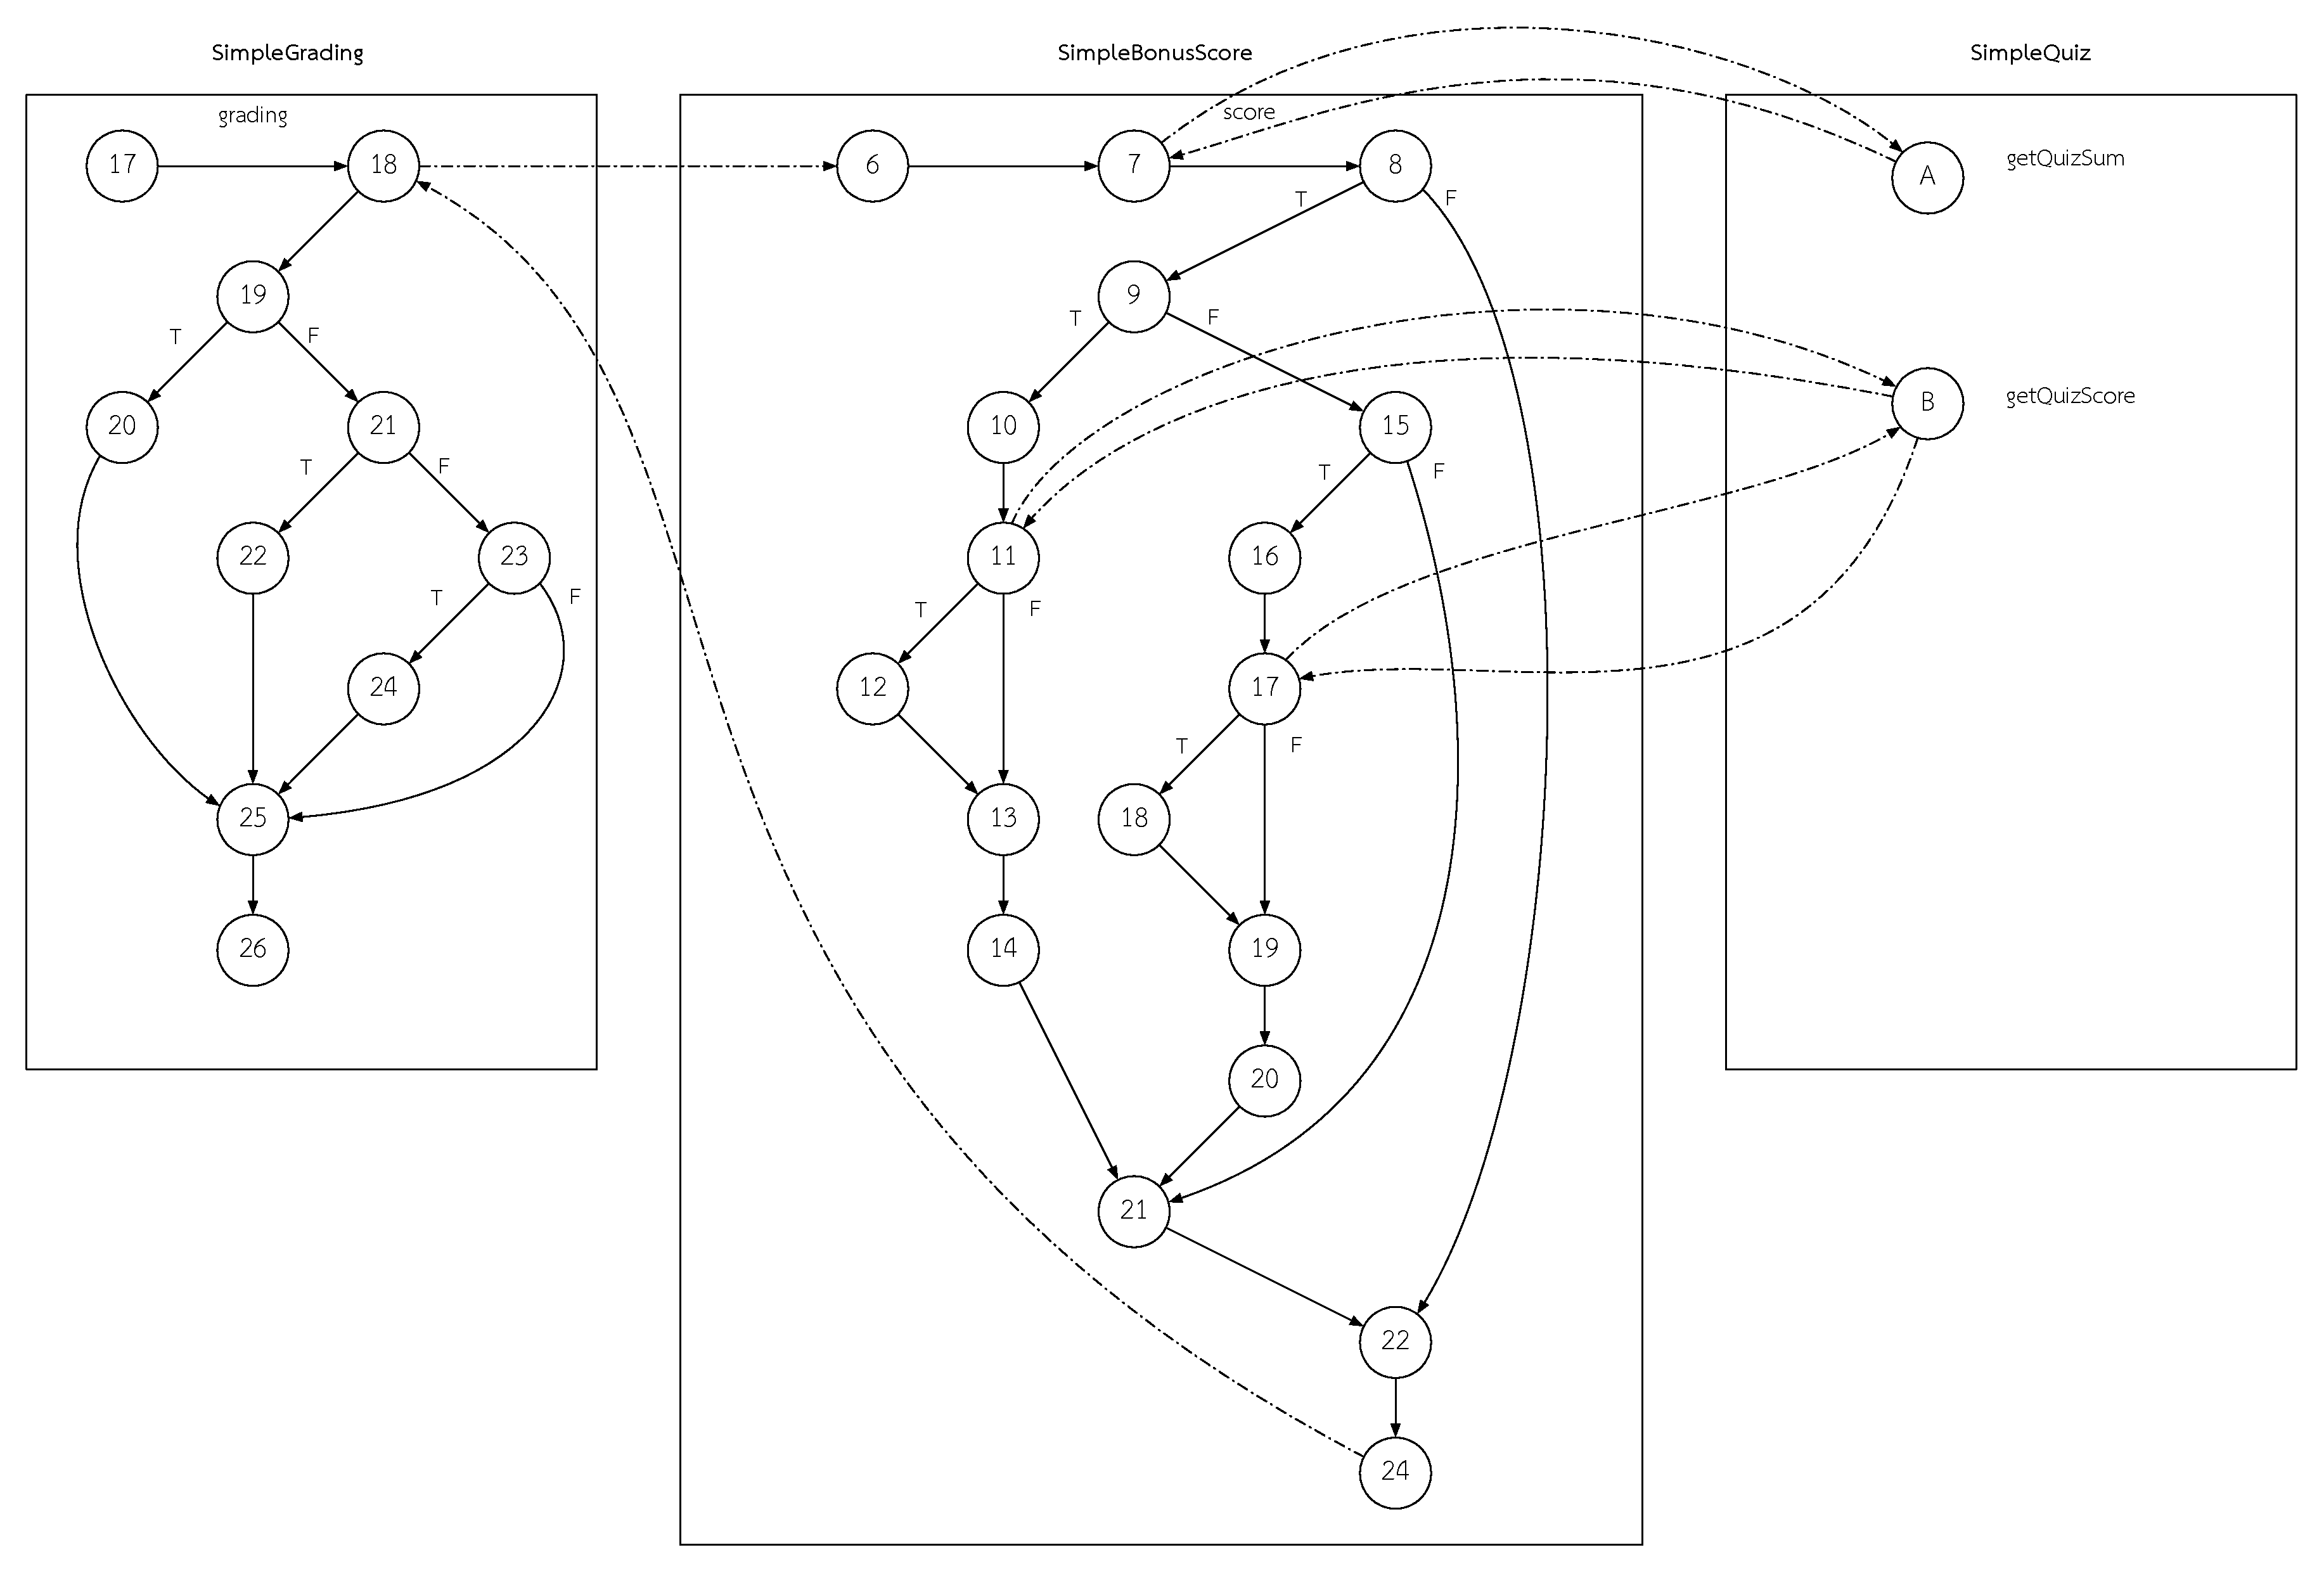
\includegraphics[width=0.9\textwidth]{test-path-selection-call-reference}
    \caption{โครงสร้างความสัมพันธ์ของ\class \code{SimpleGrading}, \code{SimpleBonusScore} และ\code{SimpleQuiz}}
    \label{fig:callreferences}
\end{sidewaysfigure}

ซึ่งมีแนวทางการเลือก{\TestPath} ดังนี้

\begin{enumerate}
    \item ให้น้ำหนักในทิศทางที่มุ่งไปยัง{\Node} ซึ่งพบการเรียกใช้งานระหว่าง{\class}ตามที่กำหนดไว้จาก{\scg}มากที่สุดเสมอ
    \item เลือก{\TestPath}ที่สั้นที่สุด (Shortest path) ก่อนเสมอ
    \item เลือก{\TestPath}ที่พบ{\PredicateNode}น้อยที่สุดก่อนเสมอ
    \item เลือก{\TestPath}ไปยังทิศที่ทำให้{\PredicateNode}มีค่าความจริงเป็นจริงก่อนเสมอ
\end{enumerate}

เมื่อพิจารณาข้อมูลกราฟดัง \figref{fig:callreferences} จะได้{\TestPath} \code{P_1} ดังนี้
\begin{equation*}
    \centering
    \code{P_1: \underbrace{17-18}_{G}-\overbrace{6-7}^{B}-\underbrace{A}_{Q}-\overbrace{7-\overline{8}-22-24}^{B}-\underbrace{18-19-20-25-26}_{G}} 
    \label{eq:exampleTestPathP1}
\end{equation*}
% \begin{equation*}
%     \centering
%     \code{P_2: \underbrace{17-18}_{G}-\overbrace{6-7-8-9-10-11}^{B}-\newline \underbrace{B}_{Q}-\overbrace{11-12-13-14-21-22-23-24}^{B}-\underbrace{18-19-20-25-26}_{G}}
% \end{equation*}

\clearpage
\subsubsection{การวิเคราะห์พารามิเตอร์และการคืนค่าของ{\method}}

แนวทางในขั้นตอนนี้จะนำ{\TestPath}ที่ได้คัดเลือกไว้ในขั้นตอนก่อนหน้านี้ (ซึ่งในที่นี้คือ \code{P_1} และ\code{P_2}) มาพิจารณาข้อมูลนำเข้า
และพารามิเตอร์ของแต่ละ{\method}ที่มีการเรียกผ่านกัน โดยจะเริ่มพิจารณาที่{\PredicateNode}ที่อยู่ในลำดับท้ายสุดของ{\TestPath}ก่อนเสมอ 
แล้วจึงนำเงื่อนไขการสร้างข้อมูลของทั้งเส้นทางมากำหนดกรอบสำหรับการสร้างข้อมูล 
ยกตัวอย่างเช่น \code{P_1} จะพบ{\PredicateNode}ทั้งสิ้น 2 {\Node} ด้วยกัน ได้แก่ {G: 19} และ \code{S: 8}
ซึ่งมีเงื่อนไขดังนี้

\begin{enumerate}
    \item[G:19] \code{student\_score < SCORE\_MINIMUM\_STATISFIED} \label{itm:studentscore}
    \item[S:8]  \code{bonus\_score > 0} \label{itm:studentid}
\end{enumerate}

โดยในขั้นตอนนี้จะนำค่าคงที่ที่เก็บไว้ในขั้นตอน {\bf \constantExtracting}} มาแทนในตัวแปร \code{SCORE\_MINIMUM\_STATISFIED} 
(\code{SCORE\_MINIMUM\_STATISFIED} มีค่าเท่ากับ \code{80}) แล้วจึงพิจารณาข้อมูลทดสอบจากเงื่อนไขข้างต้น
เพื่อสร้างกรณีทดสอบและข้อมูลทดสอบที่เข้าทดสอบ{\TestPath}ตามที่เลือกได้ โดยที่ข้อมูลที่สร้างขึ้นนั้นจะต้องทำให้เงื่อนไข 
\code{G:19} เป็นจริง (\code{True}) และเงื่อนไข \code{S:8} เป็นเท็จ (\code{False})

\subsubsection{\FirstTimeDefine{\randomTestData}{\randomTestDataEN}}
\label{sec:sub:randomTestData}

สำหรับแนวทางการดำเนินงานในขั้นตอนนี้จะรับเงื่อนไขการสร้าง{\testData}จากกระบวนการก่อนหน้าเพื่อนำมาสร้างข้อมูลทดสอบ 
เพื่อให้กรณีทดสอบสามารถทดสอบ{\TestPath}ตามที่เลือกได้ ตามวิธีการที่กำหนด \cite{XING201491, Ma2016, Heaton2000} 
หากมีพารามิเตอร์ที่ไม่ปรากฎใน{\TestPath}เป็นข้อมูลนำเข้า ให้คำนวณหาค่าความน่าจะเป็นที่จะนำค่าคงที่มาใช้ TF-IDF 
(Term Frequency-Inverse Document Frequency: TF-IDF) \cite{Ma2016} 

เมื่อพิจารณาข้อมูล\FirstTimeDefine{\MethodSignature}{\MethodSignatureEN} ของ{\method} \code{score} ของ{\class} \code{SimpleGrading} 
พบว่า{\method}นี้ต้องการพารามิเตอร์ทั้งหมด 3 ค่า ด้วยกัน คือ \code{student\_id:String}, \code{student\_score:int} และ\code{bonus\_score:int} 
แต่จากตัวแปรที่พบใน{\PredicateNode}นั้นจะมีเพียง \code{student\_score} และ\code{bonus\_score} 
คงเหลือตัวแปร \code{student\_id} ที่จะใช้การคำนวณความคล้ายด้วยวิธี TF-IDF \cite{Ma2016}
กำหนดให้ค่าที่สุ่ม{\it \randomTestData } ได้ออกมาเป็นดัง \tabpageref{tab:GRTRandom}

\begin{table}[ht!]
    \centering
    \caption{ตัวอย่าง{\randomTestData}ที่ได้}
    \label{tab:GRTRandom}
    \begin{tabular}{|l|c|c|}
        \hline
        ตัวแปร                    & ประเภทข้อมูล   & ค่าที่สุ่มได้          \\ \hline
        \code{student\_score}    & {\it int}    & {\bf 75}         \\ \hline
        \code{bonus\_score}      & {\it int}    & {\bf 0}         \\ \hline
        \code{student\_id}       & {\it String} & {\bf "IUUUSISS"} \\ \hline
    \end{tabular}
\end{table}

\subsubsection{\FirstTimeDefine{\testcaseGeneration}{\testcaseGenerationEN}}
\label{sec:sub:sub:tcGen}

ในขั้นตอนนี้จะนำข้อมูลนำเข้าที่สร้างจากกระบวนการก่อนหน้ามาสร้างกรณีทดสอบสำหรับภาษาจาวา โดยใส่{\expectedOutput} (บรรทัดที่ 7) 
จะเกิดจากการสุ่มโดยอิงตามประเภทข้อมูลที่{\method}นั้นคืนค่า ดังตัวอย่างของกรณีทดสอบภายใน {\it \testSuite} ดัง \figref{fig:junitGradingTest} ด้านล่าง

\begin{figure}[hbt!]
    \lstset{basicstyle=\small,style=thesiscodestyle}
    \lstinputlisting[language=Java]{methodology/SimpleGradingTest.java}
    \caption{กรณีทดสอบที่สร้างขึ้นจากข้อมูลทดสอบ}
    \label{fig:junitGradingTest}
\end{figure}

\clearpage
\subsection{\FirstTimeDefine{\expectedOutputAdjustment}{\expectedOutputAdjustmentEN}}
\label{sec:sub:expectedOutputAdj}

ในขั้นตอนนี้\tester จะทำหน้าที่ปรับค่า\FirstTimeDefine{\expectedOutput}{\expectedOutputEN}
แนวทางการดำเนินงานในขั้นตอนนี้จะเป็นการปรับค่าข้อมูลที่อยู่ภายในกรณีทดสอบที่ได้รับโดยนักทดสอบซอฟต์แวร์ เพื่อให้กรณีทดสอบนั้นสอดคล้องกับการทำงานที่ควรจะเป็นของโปรแกรม
มากที่สุด เนื่องจากการวิจัยครั้งนี้ยังไม่รองรับการวิเคราะห์ค่าผลลัพธ์ที่ได้จากการดำเนินงานของ{\method} ยกตัวอย่างเช่นกรณีทดสอบที่ได้จากขั้นตอนที่ 5.4 
ดัง \figref{fig:junitGradingTest} เมื่อได้ปรับการปรับค่าความคาดหวังจากนักทดสอบซอฟต์แวร์แล้วจะได้เป็นดัง{\figref{fig:junitGradingTestRefined}
ซึ่งในที่นี้นักทดสอบซอฟต์แวร์ได้ปรับค่าในบรรทัดที่ 5 โดยเปลี่ยนจาก \code{"IUUUSISS"} ให้เป็นค่า \code{"5873000021"} 
และบรรทัดที่ 7 คือค่า \code{"lorem"} เป็นค่า \code{"U"} จะได้ตัวอย่างของ {\it กรณีทดสอบพร้อมใช้งาน (ญ)} ดังนี้

\begin{figure}[hbt!]
    \lstset{style=thesiscodestyle}
    \lstinputlisting{methodology/SimpleGradingTest-Refined.java}
    \caption{กรณีทดสอบที่สร้างขึ้นจากข้อมูลทดสอบที่ปรับค่าจากนักทดสอบซอฟต์แวร์แล้ว}
    \label{fig:junitGradingTestRefined}
\end{figure}

\subsection{}

แนวทางการดำเนินงานในขั้นตอนนี้จะรับ {\it ชุดกรณีทดสอบ (ญ)} เข้าทดสอบร่วมกับ{\sourcecode}ที่ผ่าน{\it การแทรกคำสั่ง (จ)} จาก{\it ฐานข้อมูล (A)} 
และรวบรวมข้อมูลที่เกิดจากชุดคำสั่งที่แทรกไว้ ซึ่งปรากฎขึ้นระหว่างการทดสอบเข้าไว้ด้วยกันเป็น {\it ผลลัพธ์การทดสอบซอฟต์แวร์ (ฎ)} 
เพื่อใช้ตรวจสอบให้แน่ใจว่ากรณีทดสอบนั้นสามารถทดสอบ{\TestPath}ที่เลือกได้ 

\subsection{เปรียบเทียบผลลัพธ์การดำเนินงาน (8)}

ในขั้นตอนนี้จะรับ {\it ผลลัพธ์การทดสอบซอฟต์แวร์ (ฎ)} มาสร้างเส้นทางการทดสอบเทียบกับ{\TestPath}ที่ได้เลือกไว้ก่อนหน้านี้ 
เพื่อให้แน่ใจได้ว่าชุดทดสอบที่สร้างขึ้นนั้นครอบคลุม{\scg}ตาม{\TestPath}ที่กำหนดไว้


    \section{วัตถุประสงค์ของงานวิจัย}

\begin{enumerate}
    \item ศึกษาและออกแบบแนวทางการสร้างการกรณีทดสอบจาก{\scg}สำหรับภาษาจาวา เพื่อสร้างกรณีทดสอบที่ครอบคลุม{\TestPath}ระหว่าง{\CUT} อย่างน้อย 1 เส้นทาง
    \item สร้างข้อมูลทดสอบที่สอดคล้องกับ{\TestPath}ที่เลือก ด้วยวิธีการกำหนดกรอบค่าสำหรับการสุ่มข้อมูลนำเข้า
\end{enumerate}



    \section{ขอบเขตงานวิจัย}

\begin{enumerate}
    \item ข้อมูล{\scg}ที่สร้างขึ้นนั้นจะสนใจเฉพาะคลาสที่อยู่ภายในแพ็คเกจจาวา (Java package) ตามที่ผู้ใช้ระบุ 
        โดยละเว้นชุดพัฒนามาตรฐานของภาษาจาวาและชุดคำสั่งภายนอก
    \item รองรับข้อมูลนำเข้าประเภทตัวอักษร (มีชนิดข้อมูลเป็น String ในภาษาจาวา) ตัวเลข 
        (มีชนิดข้อมูลเป็น byte, short, int, long, float และ double ในภาษาจาวา) และโครงสร้างข้อมูลจำกัดเขต (มีชนิดข้อมูลเป็น enum ในภาษาจาวา) 
        ยังไม่รองรับประเภทข้อมูลเฉพาะที่สร้างขึ้นเอง
    \item รองรับโปรแกรมประยุกต์ที่พัฒนาขึ้นเพื่อใช้งานบนเครื่องคอมพิวเตอร์ส่วนบุคคล และ{\sourcecode}พัฒนาขึ้นด้วยภาษาจาวา 
        โดยไม่รวมถึงโปรแกรมประยุกต์ประเภทเว็บแอปพลิเคชัน
    \item ครอบคลุมโปรแกรมที่ทำงานเป็นลำดับ (Sequencial) ไม่ครอบคลุมการทำงานของโปรแกรมที่ทำงานเป็นภาวะพร้อมกัน (Sequencial programming)
    \item รองรับเฉพาะโปรแกรมที่มีจำนวนของไซโคลเมทิกภายในคลาสรวมกันแล้วน้อยกว่าหรือเท่ากับ 15
    \item รองรับการสร้างกรณีทดสอบที่สอดคล้องตามรูปแบบของชุดพัฒนา JUnit
    \item รองรับการดำเนินงานแบบวงวน (Loop) มากที่สุด 2 รอบ
    \item ไม่รองรับการเรียกใช้ฟังก์ชันเวียนบังเกิด (Recursion)
\end{enumerate}


    % -------------------- 
    % References section
    % -------------------- 
    \bibliographystyle{acm}
    \bibliography{references}
    % --------------------

\end{document}

